%编译链是txs:///xelatex | txs:///biber | txs:///xelatex | txs:///xelatex | txs:///view

\documentclass{beamer}
\usepackage{ctex, hyperref}
\usepackage{calligra}
\usepackage[]{amsmath}
\usepackage{amssymb}
\usepackage{annotate-equations}
\usepackage{utfsym}
\usepackage[]{adjustbox}
\usepackage{calligra}
\usepackage{extpfeil}
\usepackage{physics}
\usepackage[T1]{fontenc}
\usepackage{ragged2e}
\usepackage{simpler-wick}
\usepackage{extarrows}
\justifying\let\raggedright\justifying


\usepackage[style=alphabetic]{biblatex}  % 改用biber
\addbibresource{ref.bib}

% 清除冗余字段（期刊、出版社、页码等）
% 这样参考文献列表除了作者年份和论文题目，其它的都不会输出
\AtEveryBibitem{
	\clearlist{language}     % 清除语言字段
	\clearfield{journaltitle} % 期刊名称
	\clearfield{volume}       % 卷号
	\clearfield{number}       % 期号
	\clearfield{pages}        % 页码
	\clearlist{publisher}     % 出版社
	\clearlist{location}      % 出版地
	\clearfield{isbn}         % ISBN
	\clearfield{issn}         % ISSN
	\clearfield{note}         % 备注
	\clearfield{eprint}       % arXiv 号（二次确认）
	\clearfield{doi}
	\ifentrytype{article}{    % 针对期刊文章额外清理
		\clearfield{urldate}     % 访问日期
	}{}
}

%% 作者部分
\author{Bufan Zheng}
\title{An Introduction to Pure Spinor Formalism with application to Tree-Level String Amplitudes}
\subtitle{based on my bachelor thesis}
\institute{Department of Physics, University of Tokyo}
\date{2025年9月24日}
\usepackage{WHU}
% 调整页面左右边距
\setbeamersize{text margin left=0.3cm, text margin right=0.3cm}

\setlength{\parindent}{0pt} % 取消所有段落缩进
%自定义命令
%% 实现双重尖括号
\makeatletter
\newsavebox{\@brx}
\newcommand{\llangle}[1][]{\savebox{\@brx}{\(\m@th{#1\langle}\)}%
	\mathopen{\copy\@brx\kern-0.5\wd\@brx\usebox{\@brx}}}
\newcommand{\rrangle}[1][]{\savebox{\@brx}{\(\m@th{#1\rangle}\)}%
	\mathclose{\copy\@brx\kern-0.5\wd\@brx\usebox{\@brx}}}
\makeatother

\begin{document}

\kaishu
\begin{frame}
	\titlepage
	\vspace{-6pt}
	\begin{figure}[htpb]
		\begin{center}
			
\includegraphics[width=0.15\linewidth]{pic/UTokyo_Logo.pdf}
		\end{center}
	\end{figure}
\end{frame}
\begin{frame}
\tableofcontents[sectionstyle=show,subsectionstyle=show/shaded/hide,subsubsectionstyle=show/shaded/hide]
\end{frame}

% 在这个slide上面会出现很多公式，但是不要害怕，我只是想说明计算上有多困难，大多数技术性的细节我整理在附录里面了。

\section[Why amp?]{Why String Amplitudes？}

\begin{frame}{It's difficult to directly detect strings in the LHC, but ...}
\begin{itemize}
\item {\color{WHU} For phenomenology:}\\
	That's all we know —— string theory only has a perturbative definition.
	\begin{equation*}
		\begin{aligned}
			&S_{j_1...j_n}(k_1,\ldots,k_n)\\&=\sum_{\text{topology}}\int\frac{\left[dXdg\right]}{V_{\mathrm{diff}\times\mathrm{Weyl}}}\exp(-S_X-\lambda\chi)\prod_{i=1}^n\int d^2\sigma_ig(\sigma_i)^{1/2}V_{j_i}(k_i,\sigma_i)
		\end{aligned}
	\end{equation*}
\item {\color{WHU} For historians:}\\
	The first formula in string theory was the Veneziano amplitude, which describes the scattering of four tachyons.
	\begin{equation*}
		\begin{aligned}
			S_{D_2}&(k_1;k_2;k_3;k_4)=\frac{2ig_0^2}{\alpha^{\prime}}(2\pi)^{26}\delta^{26}(\sum_ik_i)\\&\times\left[B(-\alpha_\mathrm{o}(s),-\alpha_\mathrm{o}(t))+B(-\alpha_\mathrm{o}(s),-\alpha_\mathrm{o}(u))+B(-\alpha_\mathrm{o}(t),-\alpha_\mathrm{o}(u))\right]
		\end{aligned}
	\end{equation*}
	Where, $\alpha_o(x):=\alpha' x +1$
\end{itemize}
\end{frame}

\begin{frame}
\begin{itemize}
\item {\color{WHU} For QFT experts:}\\
	As $\alpha'$ goes to $0$, string theory reduces to QFT, making it a powerful tool for understanding QFT amplitudes. Such as KLT relation \cite{Kawai:1985xq}:
	\begin{equation*}
		\mathcal{M}_n\sim\sum_{\rho,\tau\in S_{n-3}}A_n\left(1,\rho,n-1,n|\frac{\alpha^{\prime}}{4}\right)S_{\alpha^{\prime}}(\rho|\tau)\tilde{A}_n\left(1,\tau,n,n-1|\frac{\alpha^{\prime}}{4}\right)
	\end{equation*}
	This relation implies a squaring structure, $\mathcal{A}_{\text{grav}}\sim \mathcal{A}_{\text{YM}}^2$. Furthermore, the prescription for calculating string amplitudes by integration over Riemann surfaces inspired the development of the CHY formalism in QFT \cite{Cachazo:2013iea,Cachazo:2013hca}:
	\begin{equation*}
		\mathcal{A}_n = \int_{\mathcal{M}_{0,n}} d\mu_n \mathcal{I}_\text{CHY},\quad d\mu_n:=\frac{d^n\sigma}{\mathrm{volSL}(2,\mathbb{C})}\prod_a{^{\prime}\delta}{\left(\sum_{b\neq a}\frac{s_{ab}}{\sigma_{ab}}\right)}
	\end{equation*}
	This formulation expresses QFT amplitudes in a universal language, where the dynamics of different theories are encoded solely in the integrand $\mathcal{I}_{\text{CHY}}$.
\end{itemize}
\end{frame}
\begin{frame}\label{drinfield}
	\begin{itemize}
		\item {\color{WHU} For mathematician:}\\
		Recent research has revealed that string theory amplitudes can be regarded as generating functions for number-theoretic functions, such as Multiple Zeta Values, thereby establishing a connection to number theory \cite{Broedel:2013aza}.
		
		For example, the tree-level 4-point gauge boson amplitude:
		\begin{equation*}
			\begin{aligned}
					&\mathcal{A}(1234)=A_{\text{YM}}(1234)\frac{\Gamma(1-2\alpha^{\prime}s_{12})\Gamma(1-2\alpha^{\prime}s_{23})}{\Gamma(1-2\alpha^{\prime}s_{12}-2\alpha^{\prime}s_{23})}\\
					=&\exp\left(\sum_{n-2}^\infty\frac{\color{WHU}\zeta_n}{n}(2\alpha^{\prime})^n\left[s_{12}^n+s_{23}^n-(s_{12}+s_{23})^n\right]\right)\\
					=&1-(2\alpha^{\prime})^2{\color{WHU}\zeta_2}s_{12}s_{23}+(2\alpha^{\prime})^3\zeta_3s_{12}s_{23}s_{13}\\
					&-(2\alpha^{\prime})^4{\color{WHU}\zeta_4}s_{12}s_{23}\left(s_{12}^2+\frac{1}{4}s_{12}s_{23}+s_{23}^2\right)\\
					&-(2\alpha^{\prime})^5{\color{WHU}\zeta_2\zeta_3}s_{12}^2s_{23}^2s_{13}+\frac{1}{2}(2\alpha^{\prime})^5{\color{WHU}\zeta_5}s_{12}s_{23}s_{13}(s_{12}^2+s_{23}^2+s_{13}^2)+O(\alpha^{\prime6})
			\end{aligned}
		\end{equation*}
	\end{itemize}
\end{frame}

\section[Why PS?]{RNS Formalism is not Enough}
	\begin{frame}
		To incorporate SUSY into string theory, it can be introduced either on the worldsheet or in the target spacetime.
		\begin{itemize}
			\item {\color{WHU} On the worldsheet: RNS formalism} 
			\begin{equation*}
				S_{\text{RNS}}=\frac{1}{2\pi}\int\mathrm{d}^2z\left(\frac{2}{\alpha^{\prime}}\partial X^\mu\overline{\partial}X_\mu+\psi^\mu\overline{\partial}\psi_\mu+\overline{\psi}^\mu\partial\overline{\psi}_\mu\right)+S_{\text{gh}}
			\end{equation*}
		\end{itemize}
		What is truly desired is target spacetime supersymmetry, which remains hidden in the RNS formalism. This can be made manifest through the {\color{WHU} GSO projection}. 
		
		It's easy to construct string spectrum by canonical quantization:
		\begin{table}[htbp]
			\centering
			\begin{tabular}{c|cc}
				\hline
				&Type IIA &Type IIB\\
				\hline
				$m^2=0$ 
				&\(\displaystyle
				\begin{gathered}
					|\alpha;-\rangle_{\mathrm{R}}\otimes|\alpha;+\rangle_{\mathrm{R}}\\\tilde{\psi}_{-1/2}^i|0\rangle_{\mathrm{NS}}\otimes \psi_{-1/2}^j|0\rangle_{\mathrm{NS}}\\\tilde{\psi}_{-1/2}^i|0\rangle_{\mathrm{NS}}\otimes|\alpha;+\rangle_{\mathrm{R}}\\|\dot\alpha;-\rangle_{\mathrm{R}}\otimes \psi_{-1/2}^i|0\rangle_{\mathrm{NS}}
				\end{gathered}
				\)
				&\(\displaystyle
				\begin{gathered}
					|\alpha;+\rangle_{\mathrm{R}}\otimes|\alpha;+\rangle_{\mathrm{R}}\\\tilde{\psi}_{-1/2}^i|0\rangle_{\mathrm{NS}}\otimes \psi_{-1/2}^j|0\rangle_{\mathrm{NS}}\\\tilde{\psi}_{-1/2}^i|0\rangle_{\mathrm{NS}}\otimes|\alpha;+\rangle_{\mathrm{R}}\\|\alpha;+\rangle_{\mathrm{R}}\otimes \psi_{-1/2}^i|0\rangle_{\mathrm{NS}}
				\end{gathered}
				\)\\
				\hline
			\end{tabular}
		\end{table}
	\end{frame}
	\begin{frame}
		It is also straightforward to construct vertex operators via the state operator correspondence. For example, considering the bosonic part.
		\begin{equation*}
			\alpha_{-m}^\mu\to i\left(\frac{2}{\alpha^{\prime}}\right)^{1/2}\frac{1}{(m-1)!}\partial^mX^\mu(0),\quad|0;k\rangle\to e^{ik\cdot X(0,0)}
		\end{equation*}
		The vertex operators relevant for tree-level amplitudes are listed below:
		\begin{equation*}
			U^{(-1)}(z)=\epsilon_\mu\psi^\mu(z)\mathrm{e}^{-\phi(z)}\mathrm{e}^{ik\cdot X(z)},\quad U^{(-\frac{1}{2})}(z)=u^\alpha S_\alpha(z)e^{-\frac{1}{2}\phi(z)}e^{ik\cdot X(z)}
		\end{equation*}
		Other two vertex operators with different picture number can be constructed via {\color{WHU}Picture Changing Operator (PCO)}. You can find them in the \hyperlink{vertex ops}{\color{blue} appendix}.
		
		Moreover, the relationship between unintegrated and integrated vertex operators is very simple in the RNS formalism:
		\begin{equation}\label{eq:UV}
			V(z) = c(z) U(z)
		\end{equation}
	\end{frame}
	\begin{frame}
		\begin{itemize}
		\item {\color{WHU} On the target Spacetime: GS formalism}
		\begin{equation*}
			S_{\mathrm{GS}}=\frac{1}{\pi}\int d^2z\left[\frac{1}{2}\Pi^m\overline{\Pi}_m+\frac{1}{4}\Pi_m(\theta\gamma^m\overline{\partial}\theta)-\frac{1}{4}\overline{\Pi}_m(\theta\gamma^m\partial\theta)\right]
		\end{equation*}
		\end{itemize}
		Comparing to RNS formalism, we know how to couple GS superstring with R-R flux. Actually, we can write down more general D brane action in GS formalism:
		\begin{equation*}
		S_{\text{D}_p}=-T_{\mathrm{D}p}\int d^{p+1}\sigma\sqrt{-\det(G_{\alpha\beta}+k\mathcal{F}_{\alpha\beta})}+S_{\text{CS}}
		\end{equation*}
		However, it is very difficult to covariantly quantize the GS superstring, we can {\color{WHU} only} quantize it in the light-cone gauge. The reasons for this are explained using a simple toy model in the \hyperlink{GS}{\color{blue}appendix}. Since our spacetime is required to be SR covariant, it can be anticipated that performing calculations within the GS formalism is rather challenging.
	\end{frame}
\section[PS superstring]{Pure Spinor Formalism}
\begin{frame}{Siegle's idea}
	To solve the problem related to GS superstring, Siegle introduced a new independent Grassmann odd variable $p$, proposed a modified action: \cite{siegel1986classical}
	\begin{equation*}
		S_{\mathrm{Siegel}}=\frac{1}{\pi}\int d^2z\left[\frac{1}{2}\partial X^m\overline{\partial}X_m+p_\alpha\overline{\partial}\theta^\alpha\right]+\text{c.c.}
	\end{equation*}
	However, this formalism is {\color{WHU}not} equivalent to the RNS formalism. The key point lies in the fact that their OPEs of the $SO(9,1)$ Noether currents differ:
	\begin{equation*}
		\Sigma_{\mathrm{RNS}}^{mn}=-\psi^m\psi^n,\quad\Sigma_{\mathrm{Siegel}}^{mn}=-\frac{1}{2}(p\gamma^{mn}\theta)
	\end{equation*}
	\begin{equation}\label{ope diff}
		\begin{aligned}
			\Sigma_{\mathrm{RNS}}^{mn}(z)\Sigma_{\mathrm{RNS}}^{pq}(w)&\sim\frac{\delta^{p[m}\Sigma^{n]q}(w)-\delta^{q[m}\Sigma^{n]p}(w)}{z-w}+\frac{\delta^{m[q}\delta^{p]n}}{(z-w)^2}\\
			\Sigma_{\mathrm{Siegel}}^{mn}(z)\Sigma_{\mathrm{Siegel}}^{pq}(w)&\sim\frac{\delta^{p[m}\Sigma^{n]q}(w)-\delta^{q[m}\Sigma^{n]p}(w)}{z-w}+{\color{WHU}4}\frac{\delta^{m[q}\delta^{p]n}}{(z-w)^2}
		\end{aligned}
	\end{equation}
	 Moreover, $c_{\text{Siegle}}=-22\neq 0$. This is {\color{WHU}not} a consistent string theory!
\end{frame}
\begin{frame}[allowframebreaks]{Berkovits' idea}
	Referring to \hyperlink{ope diff}{\color{blue}equation (2)}, although they are different, they exhibit very similar forms. Suppose we introduce Grassmann even ghost fields $\{\lambda_{\alpha},w^{\alpha}\}$ conjugate to $\{p_\alpha,\theta^\alpha\}$. The Lorentz current is then corrected to:
	\begin{equation*}
		M^{\mu\nu}_{\text{PS}}=\Sigma^{\mu\nu}_\text{Siegle}+N_{\text{gh}}^{\mu\nu}
	\end{equation*}
	If $N_{\text{gh}}^{\mu\nu}$ satisfy the OPE below, and $c_{\lambda}=22$, the problem is resolved: \cite{Berkovits:2000fe}
	\begin{equation*}
		\begin{aligned}
			&N^{\mu\nu}(z)N^{\rho\sigma}(w)\sim\frac{\delta^{\rho[\mu}N^{\nu]\sigma}(w)-\delta^{\sigma[\mu}N^{\nu]\rho}(w)}{z-w}-{\color{WHU}3}\frac{\delta^{m[\sigma}\delta^{\rho]\nu}}{(z-w)^2}\\
			&\Sigma^{\mu\nu}(z)N^{\rho\sigma}(w)\sim\mathrm{regular}
		\end{aligned}
	\end{equation*}
	After tedious calculation, Berkovits proposed pure spinor superstring action: 
	\begin{equation*}
		S_{\mathrm{PS}}=\frac{1}{\pi}\int d^2z\left(\frac{1}{2}\partial X^m\overline{\partial}X_m+p_\alpha\overline{\partial}\theta^\alpha-w_\alpha\overline{\partial}\lambda^\alpha\right)+\text{c.c.},\quad \lambda\gamma^\mu\lambda = 0
	\end{equation*}
	With following OPE relations: (because PS constraint, $w,\lambda$ ghost is not a free CFT.\footnote{We can use $U(5)$ decomposition of $SO(10)$ to obtain a free CFT, but it's too technical to include here, even in the appendix ...} i.e. $w_{\alpha}(z)\lambda^{\beta}(w){\color{WHU}\nsim}\frac{\delta_{\alpha}^{\beta}}{z-w}$)
	\vspace*{-4pt}
	\begin{equation*}
		\begin{gathered}
			X^\mu(z,\overline{z})X^\nu(w,\overline{w})\sim-\eta^{\mu\nu}\ln|z-w|^2,\quad d_\alpha(z)\theta^\beta(w)\sim\frac{\delta_\alpha^\beta}{z-w},\\d_\alpha(z)d_\beta(w)\sim-\frac{\gamma_{\alpha\beta}^\mu\Pi_\mu(w)}{z-w},\quad d_\alpha(z)\Pi^\mu(w)\sim\frac{(\gamma^\mu\partial\theta(w))_\alpha}{z-w},\\\begin{aligned}\Pi^\mu(z)\Pi^\nu(w)\sim-\frac{\eta^{\mu\nu}}{(z-w)^2},\quad d_\alpha(z)K\sim\frac{D_\alpha K}{z-w},\quad\Pi^m(z)K\sim-\frac{\partial^mK}{z-w}\end{aligned}\\\begin{aligned}D_\alpha=\frac{\partial}{\partial\theta^\alpha}+\frac{1}{2}(\gamma^\mu\theta)_\alpha\partial_\mu,\quad\Pi^m=\partial X^m+\frac{1}{2}(\theta\gamma^m\partial\theta)\end{aligned}\\d_{\alpha}=p_{\alpha}-\frac{1}{2}\left(\partial X^{m}+\frac{1}{4}(\theta\gamma^{m}\partial\theta)\right)(\gamma_{m}\theta)_{\alpha}
		\end{gathered}
	\end{equation*}
\end{frame}
\begin{frame}{The vertex operators}
	To obtain the vertex operators, BRST quantization is the best approach:
	\begin{equation*}
		Q_B:=\oint dz(\lambda^\alpha d_\alpha) \overset{Q_B^2=0}{\Longrightarrow}\lambda\gamma^\mu\lambda = 0 \text{  (PS constraint)}
	\end{equation*}
	The vertex operator for massless (open string) excitations can be straightforwardly constructed by computing the BRST cohomology:
	\begin{equation*}
		\begin{aligned}
			U(z)&=\partial\theta^\alpha A_\alpha(X,\theta)+A_m(X,\theta)\Pi^m+d_\alpha W^\alpha(X,\theta)+\frac{1}{2}N_{mn}F^{mn}(X,\theta)\\
			V(z)&=\lambda^\alpha A_\alpha(X,\theta),\quad\{A_{\alpha/m},W^\alpha,F^{mn}\}\mathrm{~(a.k.a.~}K)\in10\text{D SYM}
		\end{aligned}
	\end{equation*}
	Details on the 10D SYM superfields are provided in the  \hyperlink{10d sym}{\color{blue} appendix}. These operators can then be used to compute disk amplitudes:
	\begin{equation}\label{disk}
		\mathcal{A}(P)=\int_{D(P)}dz\langle\langle V_1(\hat z_1)U_2(z_2)\ldots U_{n-2}(z_{n-2})V_{n-1}(\hat z_{n-1})V_n(\hat z_n)\rangle\rangle
	\end{equation}
	A simple example can be found in the \hyperlink{3-pt}{\color{blue} appendix}.
	% 给一个三点的计算例子在附录
\end{frame}
\begin{frame}{Pure spinor formalism vs. RNS formalism (Cons)}
\only<1>{	
	\begin{itemize}
		\item {\color{WHU} Non-trivial relation between $U$ and $V$.} 
		\begin{equation*}
				\text{PS: }\partial V(z) = Q_B U(z),\quad\text{RNS: }V(z) = c(z) U(z)
		\end{equation*}
		\item {\color{WHU} More complicated vertex operators.} Unintegrated vertex operator for the first massive level $\alpha'm^2=1$ was found in 2002 \cite{Berkovits:2002qx}
		\begin{equation*}
			\begin{aligned}
				V&=\partial\lambda^\alpha A_\alpha(x,\theta)+:\partial\theta^\beta\lambda^\alpha B_{\alpha\beta}(x,\theta):+:d_\beta\lambda^\alpha C_\alpha^\beta(x,\theta):\\
				&+:\Pi^m\lambda^\alpha H_{m\alpha}(x,\theta):+:J\lambda^\alpha E_\alpha(x,\theta):+:N^{mn}\lambda^\alpha F_{\alpha mn}(x,\theta):
			\end{aligned}
		\end{equation*}
		But, it was not until 2018 that the integrated vertex operator was explicitly constructed\cite{Chakrabarti:2018mqd}:
		\begin{equation*}
			\begin{aligned}
				U&=:\Pi^m\Pi^nF_{mn}:+:\Pi^md_\alpha F_m^\alpha:+:\Pi^m\partial\theta^\alpha G_{m\alpha}:+:\Pi^mN^{pq}F_{mpq}:\\&+:d_\alpha d_\beta K^{\alpha\beta}:+:d_\alpha\partial\theta^\beta F^\alpha{}_\beta:+:d_\alpha N^{mn}G^\alpha{}_{mn}:+:\partial\theta^\alpha\partial\theta^\beta H_{\alpha\beta}:\\&+:\partial\theta^\alpha N^{mn}H_{mn\alpha}:+:N^{mn}N^{pq}G_{mnpq}:
			\end{aligned}
		\end{equation*}
	\end{itemize}
}
	\only<2>{
		Where,
		\vspace{-15pt}
		\begin{columns}[t]
			\scriptsize 
			\column{0.40\textwidth}
			\begin{equation*}
				\begin{aligned}
				F_{mn} &= -\frac{18}{\alpha'}\,G_{mn},\\[4pt]
				F_{mpq} &= \frac{12}{(\alpha')^2}B_{mpq} - \frac{36}{\alpha'}\partial_{[p}G_{q]m},\\[4pt]
				F^{\alpha}{}_{\beta} &= -\frac{4}{\alpha'}(\gamma^{mnpq})^{\alpha}{}_{\beta}\,\partial_m B_{npq},\\[4pt]
				H_{\alpha\beta} &= \frac{2}{\alpha'}\gamma^{mnp}_{\alpha\beta}B_{mnp},\\[6pt]
				G_{mnpq} &= \frac{4}{(\alpha')^2}\partial_{[m}B_{n]pq}
				+ \frac{4}{(\alpha')^2}\partial_{[p}B_{q]mn}
				- \frac{12}{\alpha'}\partial_{[p}\partial_{[m}G_{n]q]}
				\end{aligned}
			\end{equation*}
			\column{0.60\textwidth}
			\begin{equation*}
			\begin{aligned}
				F_{m}{}^{\alpha} &= \frac{288}{\alpha'}(\gamma^r)^{\alpha\beta}\partial_r\Psi_{m\beta},\quad G_{m\alpha} = -\frac{432}{\alpha'}\Psi_{m\alpha}\\[4pt]
				K^{\alpha\beta} &= -\frac{1}{(\alpha')^2}\gamma^{\alpha\beta}_{mnp}B^{mnp},\\[4pt]
				G^{\alpha}{}_{mn} &= \frac{48}{(\alpha')^2}\gamma^{\alpha\sigma}{}_{[m}\Psi_{n]\sigma}
				+ \frac{192}{\alpha'}\gamma^{\alpha\sigma}{}_{r}\partial^{r}\partial_{[m}\Psi_{n]\sigma},\\[6pt]
				H_{mn\alpha} &= -\frac{576}{\alpha'}\partial_{[m}\Psi_{n]\alpha}
				- \frac{144}{\alpha'}\partial^{q}\bigl((\gamma_{q[m})_{\ \alpha}{}^{\sigma}\Psi_{n]\sigma}\bigr),\\[6pt]
			\end{aligned}
			\end{equation*}
		\end{columns}
		\vspace{12pt}
		To handle these complex formulae, several new techniques have been developed recently \cite{Kashyap:2024qor}\cite{Mafra:2024fiy}.
	}
\end{frame}
\begin{frame}{Pure spinor formalism vs. RNS formalism (Pros)}
	% 这里引用的文献是AdS PS里面的顶角算符构造
	\begin{itemize}
		\item {\color{WHU} Powerful in amplitude calculations.} Compared to the hundred-page computation of the four-point two-loop amplitude in the RNS formalism \cite{hundred}, the pure spinor formalism requires only a ten-page calculation \cite{ten}. The results were shown to be equivalent \cite{equiv}.
		
		{\color{WHU}Note:} It's still not clear how to deal with subtleties about multiloop ($\ell\geq 3$) amplitudes. 
		\item {\color{WHU} The amplitudes are manifestly SUSY and Lorentz invariant.} The pure spinor formalism computes super-amplitudes directly, whereas the RNS formalism only calculates their components.
		\item {\color{WHU} String in R-R backgrounds can be described by PS formalism.} Since the pure spinor formalism manifest spacetime supersymmetry, it can, {\color{WHU} in principle}, be used to analyze superstrings in AdS backgrounds\cite{Berkovits:2000yr}. For further discussion, see \hyperlink{comments}{\color{blue}Comments}.
	\end{itemize}
\end{frame}

\section[Disk amp]{Tree-Level Scattering Amplitudes}
\begin{frame}[allowframebreaks]{Compute OPEs ($n=2$)}
The challenge involves computing OPEs between vertex operators, e.g. for 2 points:
\begin{scriptsize}
\begin{equation*}
	\begin{gathered}
		V_1(z_1)U_2(z_2)\sim z_{12}^{-k_1\cdot k_2}\frac{L_{12}(z_2)}{z_{12}},\quad L_{12}:=-A_2^m(\lambda\gamma_mW_1)-V_2(k_2\cdot A_1)+Q_B(A_2W_1)\\
		\begin{aligned}
			U_1(z_1)U_2&(z_2)\sim z_{12}^{-k_1\cdot k_2-1}\Big(\partial\theta^\alpha\bigg[(k_1\cdot A_2)A_\alpha^1-(k_2\cdot A_1)A_\alpha^2+D_\alpha A_\beta^2W_1^\beta-D_\alpha A_\beta^1W_2^\beta\bigg]\\
			&+\Pi^m\bigg[(k_1\cdot A_2)A_m^1-(k_2\cdot A_1)A_m^2+k_m^2(A_2W_1)-k_m^1(A_1W_2)-(W_1\gamma_mW_2)\\
			&+d_\alpha\left[(k_1\cdot A_2)W_1^\alpha-(k_2\cdot A_1)W_2^\alpha+\frac{1}{4}(\gamma^{mn}W_1)^\alpha F_{mn}^2-\frac{1}{4}(\gamma^{mn}W_2)^\alpha F_{mn}^1\right]\\
			&+\frac{1}{2}N^{mn}\Big[(k_1\cdot A_2)F_{mn}^1-(k_2\cdot A_1)F_{mn}^2-2k_m^{12}(W_1\gamma_nW_2)+2F_{ma}^1F_{na}^2\Big]\Big)\\
			&+ (1+k_1\cdot k_2)z_{12}^{-k_1\cdot k_2-2}\left[(A_1W_2)+(A_2W_1)-(A_1\cdot A_2)\right]
		\end{aligned}
	\end{gathered}
\end{equation*}
\end{scriptsize}
The plane wave factors $:e^{ik\cdot X}:$ are dropped. Their contribution is restored via the Koba-Nielsen factors in the final amplitudes.

Surprisingly, if we define:
\vspace{-6pt}
\begin{small}
\begin{equation*}
	\begin{aligned}
		&A_{\alpha}^{12}=\frac{1}{2}\left[A_{\alpha}^{2}(k_{2}\cdot A_{1})+A_{2}^{m}(\gamma_{m}W_{1})_{\alpha}-(1\leftrightarrow2)\right]\\&\begin{aligned}A_{12}^m=\frac{1}{2}\left[A_2^m(k_2\cdot A_1)+A_p^1F_2^{pm}+(W_1\gamma^mW_2)-(1\leftrightarrow2)\right]\end{aligned}\\&W_{12}^{\alpha}=\frac{1}{4}(\gamma_{mn}W_{2})^{\alpha}F_{1}^{mn}+W_{2}^{\alpha}(k_{2}\cdot A_{1})-(1\leftrightarrow2)\\&F_{12}^{mn}=F_{2}^{mn}(k_{2}\cdot A_{1})+\frac{1}{2}F_{2}^{[m}F_{1}^{n]p}+k_{1}^{[m}(W_{1}\gamma^{n]}W_{2})-(1\leftrightarrow2)
	\end{aligned}
\end{equation*}
\end{small}
After dropping some BRST-exact or total derivative terms:
\vspace{-6pt}
\begin{equation*}
	U_1(z_1)U_2(z_2)\sim\frac{U_{12}(z_2)}{z_{12}},\quad V_1(z_1)U_2(z_2)\sim\frac{V_{12}(z_2)}{z_{12}}
\end{equation*}
Here $U_{12}$ and $V_{12}$ is defined by replacing superfields $K_\alpha$ with {\color{WHU}multi-particle superfields} $K_\alpha^{12}$.
\end{frame}
\begin{frame}{Compute OPEs ($n\geq 2$)}
This rule generalizes to higher points using Lie polynomial notation:
\begin{equation*}
	U_{[[1,2],3]}\leftrightarrow ((U_1 U_2) U_3),\quad U_{[[1,2],[3,4]]}\leftrightarrow ((U_1 U_2) (U_3 U_4))
\end{equation*}
The game continues:
\begin{equation*}
	V_A(z_a)U_B(z_b)\sim\frac{V_{[A,B]}(z_b)}{z_{ab}},\quad U_A(z_a)U_B(z_b)\sim\frac{U_{[A,B]}(z_b)}{z_{ab}}
\end{equation*}
\only<1>{
	In Lorentz gauge $\partial\cdot A^P=0$: \cite{Lee:2015upy}
	\begin{small}
	\begin{equation*}
		\begin{aligned}
			\hat{A}_{\alpha}^{[P,Q]}&=\frac{1}{2}\left[\hat{A}_{\alpha}^{Q}(k_{Q}\cdot\hat{A}_{P})+\hat{A}Q^{m}(\gamma_{m}\hat{W}_{P})\alpha-(P\leftrightarrow Q)\right]\\
			\hat{A}_{[P,Q]}^{m}&=\frac{1}{2}\left[\hat{A}_{Q}^{m}(k_{Q}\cdot\hat{A}_{P})+\hat{A}_{n}^{P}\hat{F}_{Q}^{nm}+(\hat{W}_{P}\gamma^{m}\hat{W}_{Q})-(P\leftrightarrow Q)\right]\\
			\hat{W}_{[P,Q]}^{\alpha}&=\frac{1}{4}\hat{F}_{P}^{rs}(\gamma_{rs}\hat{W}_{Q})^{\alpha}+\frac{1}{2}(k_{Q}\cdot\hat{A}_{P})\hat{W}_{Q}^{\alpha}+\frac{1}{2}\hat{W}_{Q}^{m\alpha}\hat{A}_{m}^{P}-(P\leftrightarrow Q)\\
			\hat{F}_{[P,Q]}^{mn}&=\frac{1}{2}\left[\hat{F}_{Q}^{mn}(k_{Q}\cdot\hat{A}_{P})+\hat{F}_{Q}^{p\mid mn}\hat{A}_{p}^{p}+\hat{F}_{Q}^{[m}\hat{F}_{P}^{n]r}-2\gamma_{\alpha\beta}^{[m}\hat{W}_{P}^{n]\alpha}\hat{W}_{Q}^{\beta}-(P\leftrightarrow Q)\right]
		\end{aligned}
	\end{equation*}
	\end{small}
}
\only<2>{
	These rules allow reducing OPEs to three-point functions like $\left\langle{V^3}\right\rangle$ e.g.:
	\begin{equation*}
	\begin{aligned}
		V_{1}(z_{1})U_{2}(z_{2})&V_{3}(z_{3})V_{4}(\infty)=\wick{\c V_1\c U_2V_3V_4}+\wick{V_1\c U_2\c V_3V_4}+\wick{V_1\c U_2V_3\c V_4}\\&\cong\frac{V_{[1,2]}(z_1)}{z_{12}}V_3(z_3)V_4(\infty)+V_1(z_1)\frac{V_{[2,3]}(z_3)}{z_{23}}V_4(\infty)\\&\cong\frac{V_{12}V_3V_4}{z_{12}}+\frac{V_1V_{32}V_4}{z_{32}}
	\end{aligned}
	\end{equation*}
}
\end{frame}
\begin{frame}{Final result}
	% 把M^3表达的式子给在附录
	% 引用文献说明自由李代数结构的出现
	Using wick contraction to reduce n-pt function:\footnote{We use the Dynkin bracket notation, $V_P:=V_{\ell(P)}$, $\ell(123\ldots n):=[\ell(123\ldots n-1),n]$}\cite{Mafra:2011nv}\cite{Mafra:2011nw}
	{\footnotesize
	\begin{equation}\label{eq:n-pt}
		\boxed{\mathcal{A}_n(P)=(2\alpha^{\prime})^{n-3}\int d\mu_P^n\sum_{AB=23\ldots n-2}\langle(V_{1A}\mathcal{Z}_{1A})(V_{(n-1)\tilde{B}}\mathcal{Z}_{n-1,\tilde{B}})V_n\rangle+\mathrm{perm}}
	\end{equation}
	}
	\begin{small}
	\begin{equation*}
		\mathcal{Z}_{123\cdots p}:=\frac{1}{z_{12}z_{23}\cdots z_{p-1,p}},\quad\int d\mu_{P}^{n}:=\int_{D(P)}dz_{2}dz_{3}\cdots dz_{n-2}\prod_{1\leq i<j}^{n-1}\left|z_{ij}\right|^{-2\alpha^{\prime}s_{ij}}
	\end{equation*}
	\end{small}
	We can use $SL(2,\mathbb{C})$ invariance to fix $\{z_1,z_{n-1},z_n\}$ to $\{0,1,\infty\}$ or $\{0,\infty,1\}$, depending on the ordering $P$. Here, $\left\langle\cdots\right\rangle$ denotes integration over the ghost fields ${\lambda,\theta}$ with the measure $\left\langle \lambda^3\theta^5\right\rangle=2880$.\footnote{See the \hyperlink{3-pt}{\color{blue}appendix} regarding the computation of the three-point amplitude.} This calculation is feasible, and further details can be found in \cite{Mafra:2022wml}. The connection with the {\color{WHU} free Lie algebra} is also discussed.
\end{frame}
\begin{frame}{The relation between 10D SYM amplitudes}
	Open string amplitudes $\xlongrightarrow{\alpha'\to 0}$ 10D SYM amplitudes:
	\begin{small}
		\begin{equation*}
			\begin{aligned}
				\mathcal{A}_n(P)&=(2\alpha^{\prime})^{n-3}\int d\mu_P^n\left[\prod_{k=2}^{n-2}\sum_{m=1}^{k-1}\frac{s_{mk}}{z_{mk}}A^{\text{YM}}_n(1,2,\ldots,n)+\mathrm{perm}(2,3,\ldots,n-2)\right]\\
				&\xlongequal{P=\{1,R,n-1,n\}} \sum_{Q\in S_{n-3}}F_R{}^Q(\alpha^{\prime})A^{\text{YM}}_n(1,Q,n-1,n)
			\end{aligned}
		\end{equation*}
	\end{small}
	Where, $s_{ij}:=p_i\cdot p_j$ and,
	\begin{equation*}
		\begin{aligned}
			F_{R}{}^{Q}(\alpha^{\prime}):=&(2\alpha^{\prime})^{n-3}\int d\mu_{R}^{n}\frac{s_{1q_{2}}}{z_{1q_{2}}}\left(\frac{s_{1q_{3}}}{z_{1q_{3}}}+\frac{s_{q_{2}q_{3}}}{z_{q_{2}q_{3}}}\right)\times\left(\frac{s_{1q_{4}}}{z_{1q_{4}}}+\frac{s_{q_{2}q_{4}}}{z_{q_{2}q_{4}}}+\frac{s_{q_{3}q_{4}}}{z_{q_{3}q_{4}}}\right)\\&\times\left(\frac{s_{1q_{n-2}}}{z_{1q_{n-2}}}+\frac{s_{q_{2}q_{n-2}}}{z_{q_{2}q_{n-2}}}+\cdots+\frac{s_{q_{n-3}q_{n-2}}}{z_{q_{n-3}q_{n-2}}}\right)\xlongrightarrow{\alpha'\to 0}\delta_{R}{}^{Q}
		\end{aligned}
	\end{equation*}
	Its $\alpha'$-expansion is related to {\color{WHU} Drinfield associator}, generating series of MZVs, as mentioned in \hyperlink{drinfield}{\color{blue}Sec. 1}.
\end{frame}
\begin{frame}[allowframebreaks]{SYM tree amplitudes from the cohomology of pure spinor superspace}
	SYM tree amplitudes can be rewritten in PS language: \cite{Mafra:2010jq}
	\begin{equation*}
		A_{n}^{\text{YM}}(P,n)=\sum_{XY=P}\langle M_{X}M_{Y}M_{n}\rangle
	\end{equation*}
		Here, $M_P$ is called the {\color{WHU}Berends–Giele current}\footnote{The original concept of the BG current comes from off-shell recursion relations of YM amplitudes.\cite{Berends:1987me}}, its exact definition can be found in \cite{Mafra:2022wml}. After integrating out zero modes:
	\begin{equation*}
		\langle M_XM_YM_Z\rangle=\frac{1}{2}\mathfrak{e}_X^m\mathfrak{f}_Y^{mn}\mathfrak{e}_Z^n+(\mathfrak{X}_X\gamma_m\mathfrak{X}_Y)e_Z^m+\mathrm{cyc}(XYZ)
	\end{equation*}
	\begin{small}
	\begin{equation*}
		\begin{aligned}
			&\mathfrak{e}_{P}^{m}=\frac{1}{s_{P}}\sum_{XY=P}\mathfrak{e}_{[X,Y]}^{m},\quad
			\mathfrak{e}_{[X,Y]}^{m}:=\frac{1}{2}\left[\mathfrak{e}_{Y}^{m}(k_{Y}\cdot\mathfrak{e}_{X})+\mathfrak{e}_{n}^{X}\mathfrak{f}_{Y}^{nm}+(\mathfrak{X}_{X}\gamma^{m}\mathfrak{X}_{Y})-(X\leftrightarrow Y)\right]\\
			&\mathfrak{X}_{P}^{\alpha}=\frac{1}{s_{P}}\sum_{XY=P}\mathfrak{X}_{[X,Y]}^{\alpha}\quad
			\mathfrak{X}_{[X,Y]}^{\alpha}:=\frac{1}{2}(k_{X}^{p}+k_{Y}^{p})\gamma_{p}^{\alpha\beta}\left[\mathfrak{e}_{X}^{m}(\gamma_{m}\mathfrak{X}_{Y})_{\beta}-\mathfrak{e}_{Y}^{m}(\gamma_{m}\mathfrak{X}_{X})_{\beta}\right]\\
			&\mathfrak{f}_{P}^{mn}:=k_{P}^{m}\mathfrak{e}_{P}^{n}-k_{P}^{n}\mathfrak{e}_{P}^{m}-\sum_{XY=P}(\mathfrak{e}_{X}^{m}\mathfrak{e}_{Y}^{n}-\mathfrak{e}_{X}^{n}\mathfrak{e}_{Y}^{m}),\quad \mathfrak{e}_1^n := e_1^n,\quad\mathfrak{X}_1^n:=\chi_1^n
		\end{aligned}
	\end{equation*}
	\end{small}
	% GGT是一个mma程序包，是依赖于closed formulae计算的
	This gives a new recursive formula for SYM tree amplitudes, fully constructed via a {\color{WHU}stringy approach}. Moreover, as discussed in \cite{Badger:2012uz} and \cite{Giele:2010ks}, Berends–Giele currents lead to fast numerical evaluation of amplitudes.
	\begin{columns}[b] % [T] 顶部对齐
		\begin{column}{0.48\textwidth} % 留出间距
			\centering
			\adjustbox{width=\linewidth, height=3cm, keepaspectratio, margin=0pt}{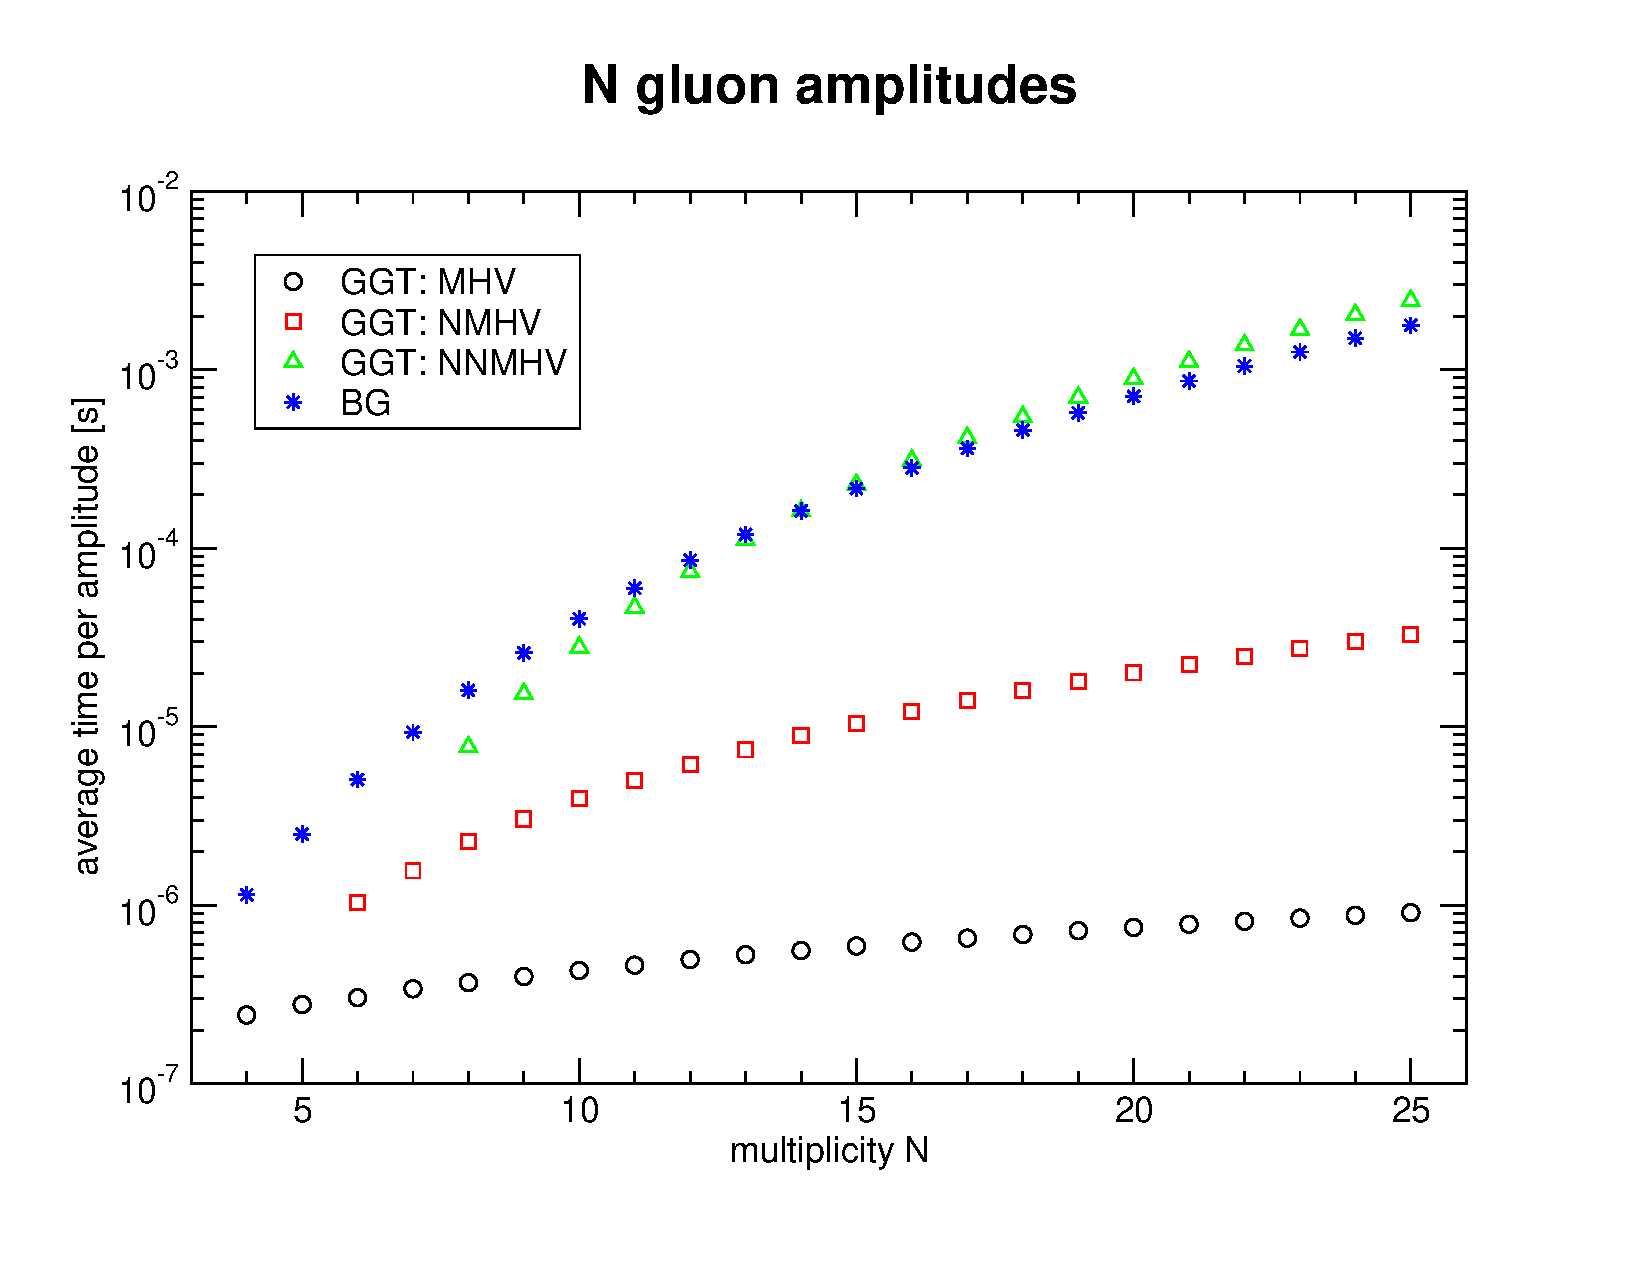
\includegraphics[width=0.9\linewidth]{pic/gluons.pdf}}% 调整图片宽度
		\end{column}
		\begin{column}{0.48\textwidth}
			\centering
			\adjustbox{width=\linewidth, height=3cm, keepaspectratio, margin=0pt}{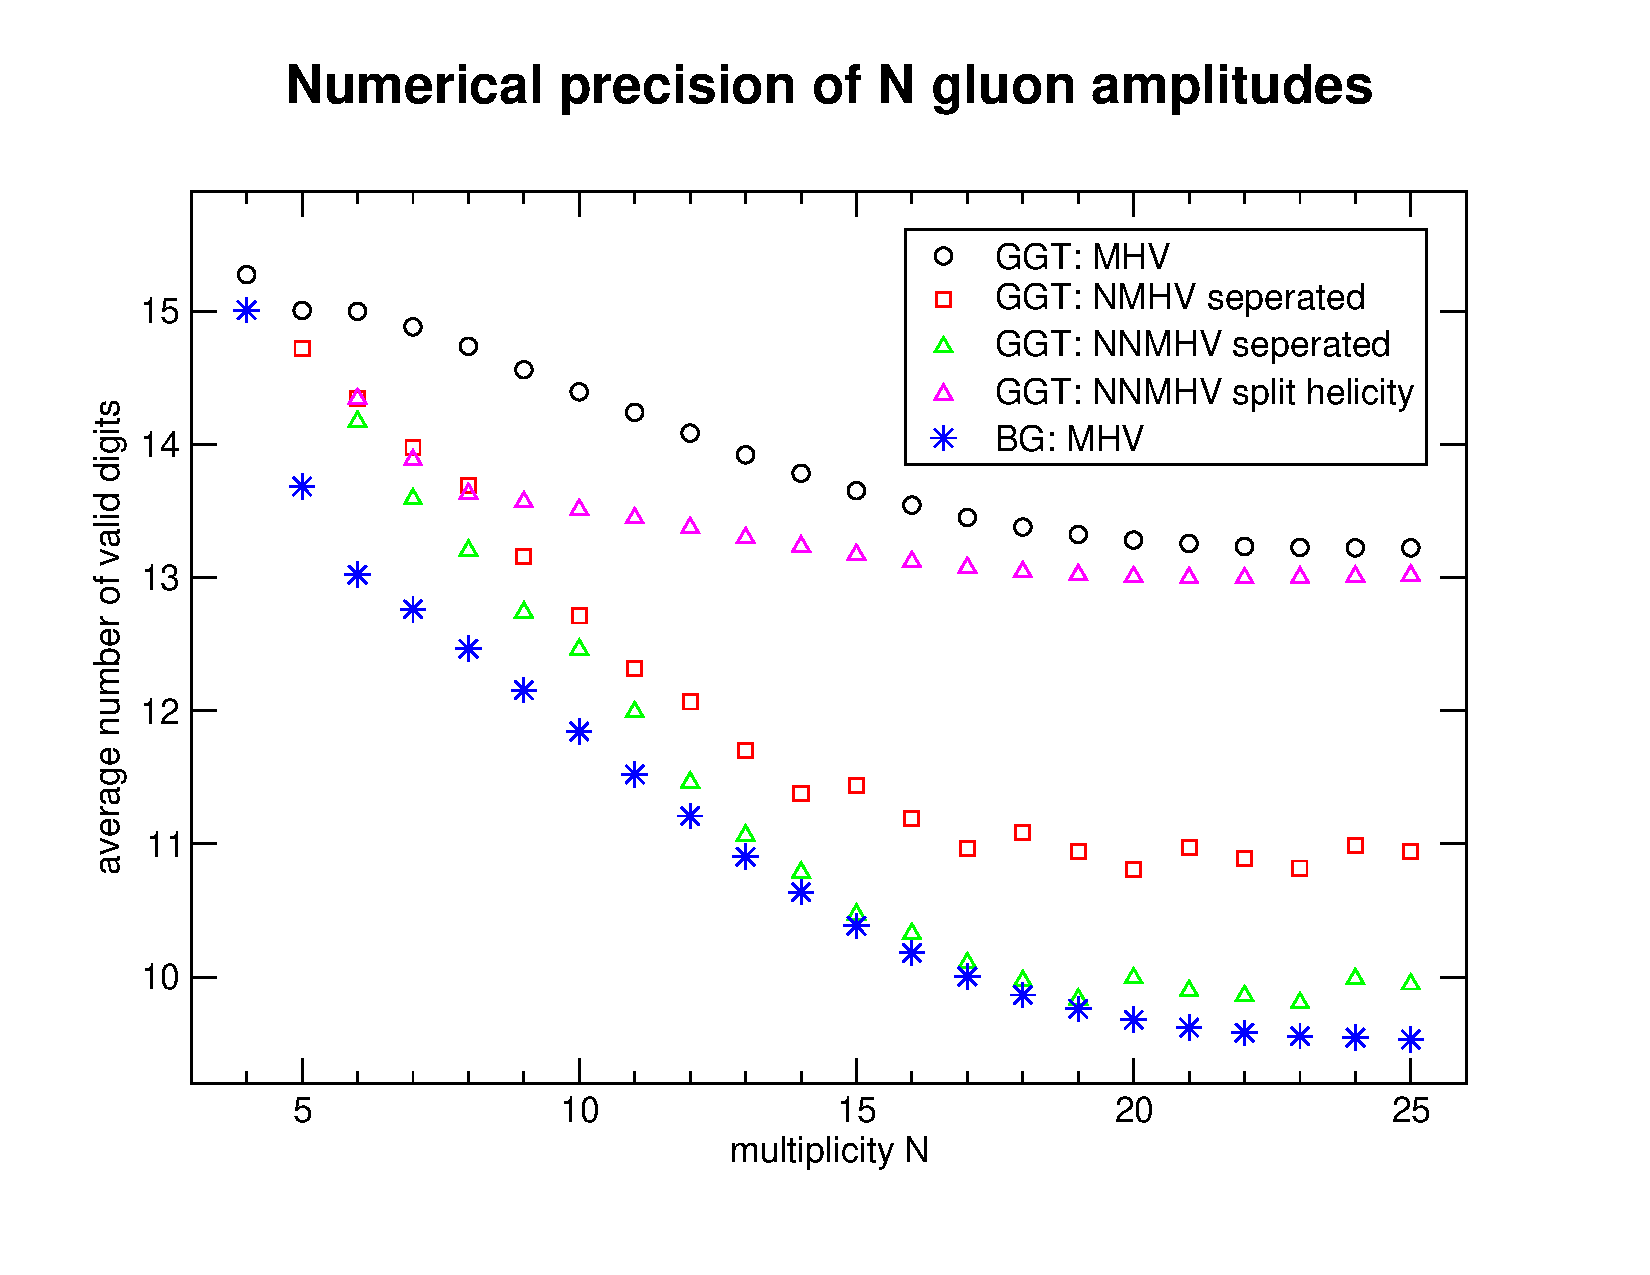
\includegraphics[width=0.9\linewidth]{pic/accuracy_gluons.pdf}}
		\end{column}
	\end{columns}
	In this representation of SYM amplitudes, relations among color-ordered partial amplitudes such as Kleiss–Kuijf and BCJ relations can also be easily derived using {\color{WHU}Ree's theorem} from free Lie algebra.\cite{Frost:2020eoa}
\end{frame}
\section[BCJ numerator]{Construct BCJ Numerator of 10d SYM Theory*}
\begin{frame}{Color-Kinematic duality: trivalent encoding}
	The full color-dressed n-point tree amplitude of Yang–Mills theory can be conveniently organized in terms of diagrams with only cubic vertices: 
	\begin{equation*}
		A_n=\sum_{i\in\Gamma_n}\frac{c_iN_i}{D_i}
	\end{equation*}
	{\color{WHU}Tips:} Why cubic vertices only?
	\begin{figure}
		\centering
		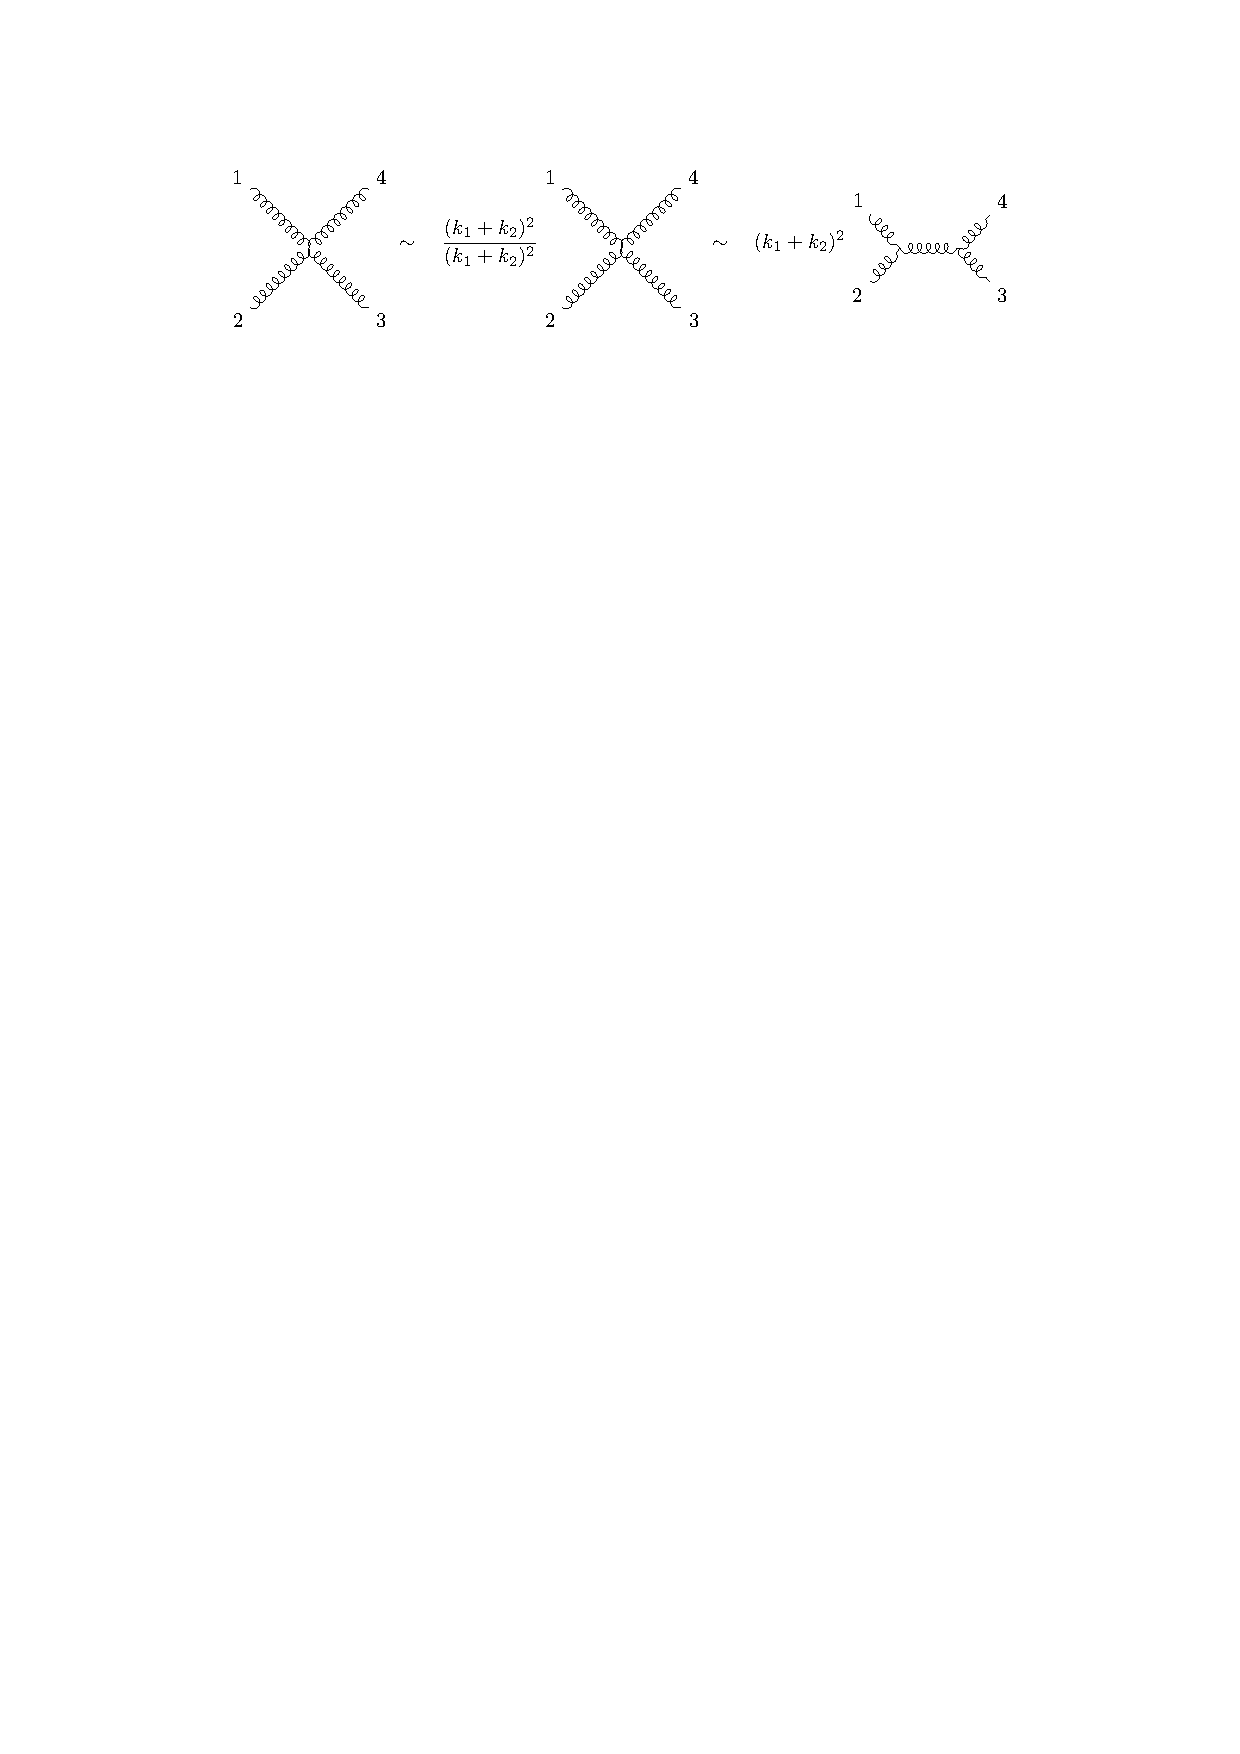
\includegraphics[width=0.8\linewidth]{pic/eq_feyn.pdf}
	\end{figure}
	The propagators $\{D_i\}$ and color factors $\{c_i\}$ are straightforward to obtain from the diagrams. However, constructing the kinematic numerators $\{N_i\}$ is non-trivial.
\end{frame}
\begin{frame}{Color-Kinematics duality: BCJ numerators}
	\cite{Bern:2008qj} showed that there exists a representation in which the kinematic numerators $\{N_i\}$ obey the same algebraic relations as the color factors $\{c_i\}$:
	\begin{figure}
		\centering
		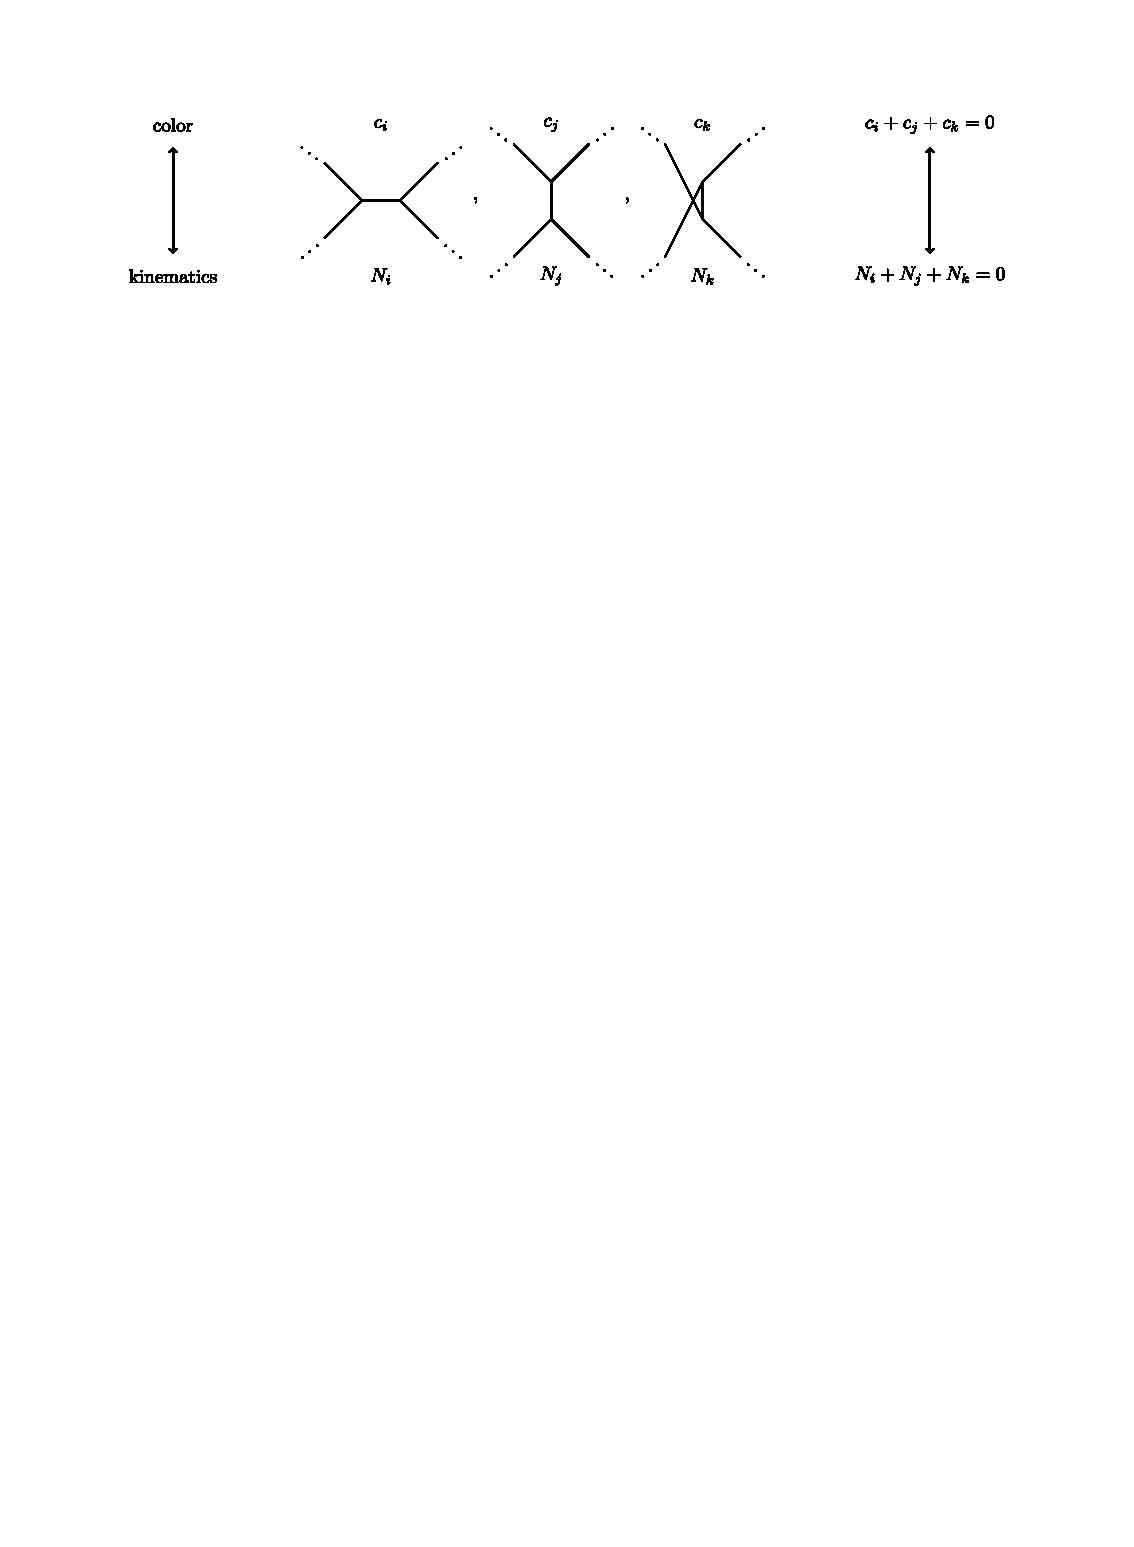
\includegraphics[width=0.90\linewidth]{pic/jacob.pdf}
	\end{figure}
	i.e., both satisfy the Jacobi identity, as well as anti-symmetry. These special (but not unique) kinematic numerators are known as {\color{WHU}BCJ numerators}.
	
	\setlength{\parindent}{2em}At tree level, BCJ numerators can be constructed through various methods, you will encounter a stringy approach later. While this duality is {\color{WHU}conjectured} to hold at loop level based on substantial evidence, a complete proof remains an open problem.
\end{frame}
\begin{frame}{Double copy relations}
	More exciting, once this is imposed, gravity amplitudes
	are obtained using two copies of gauge theory BCJ numerators: \cite{Bern:2010ue}
	\begin{equation*}
		A_n^\text{gauge}=\sum_{i\in\Gamma_n}\frac{c_iN_i}{D_i}
		\xLongrightarrow[\text{Loop }\exists\{N_i\}^\text{BCJ}\text{ ?}]{\text{Tree }\exists\{N_i\}^\text{BCJ}\, \checkmark}
		M_n^{\text{gravity}}=\sum_{i\in\Gamma_n}\frac{N_iN_i}{D_i}=\sum_{i\in\Gamma_n}\frac{N_i\tilde{N_i}}{D_i}
	\end{equation*}
	Here, ${N_i} \neq {\tilde{N}_i}$ indicates that the BCJ numerators for the "left-moving" and "right-moving" gauge theories need not be identical. In fact, the KLT relations serve as a specific realization of the double copy progaram, enabling the construction of BCJ numerators for tree-level YM theory.\cite{Carrasco:2015iwa}
	
	\setlength{\parindent}{2em}However, this remains a conjecture at the loop level and has not been proven untile now. By the way, this property is not an accident of few very special theories, but extends to large classes of gravitational and non-gravitational theories. More details can be fund in \cite{Bern:2019prr}. 
\end{frame}
\begin{frame}{Web of double copy constructible theories}
	\begin{figure}
		\centering
		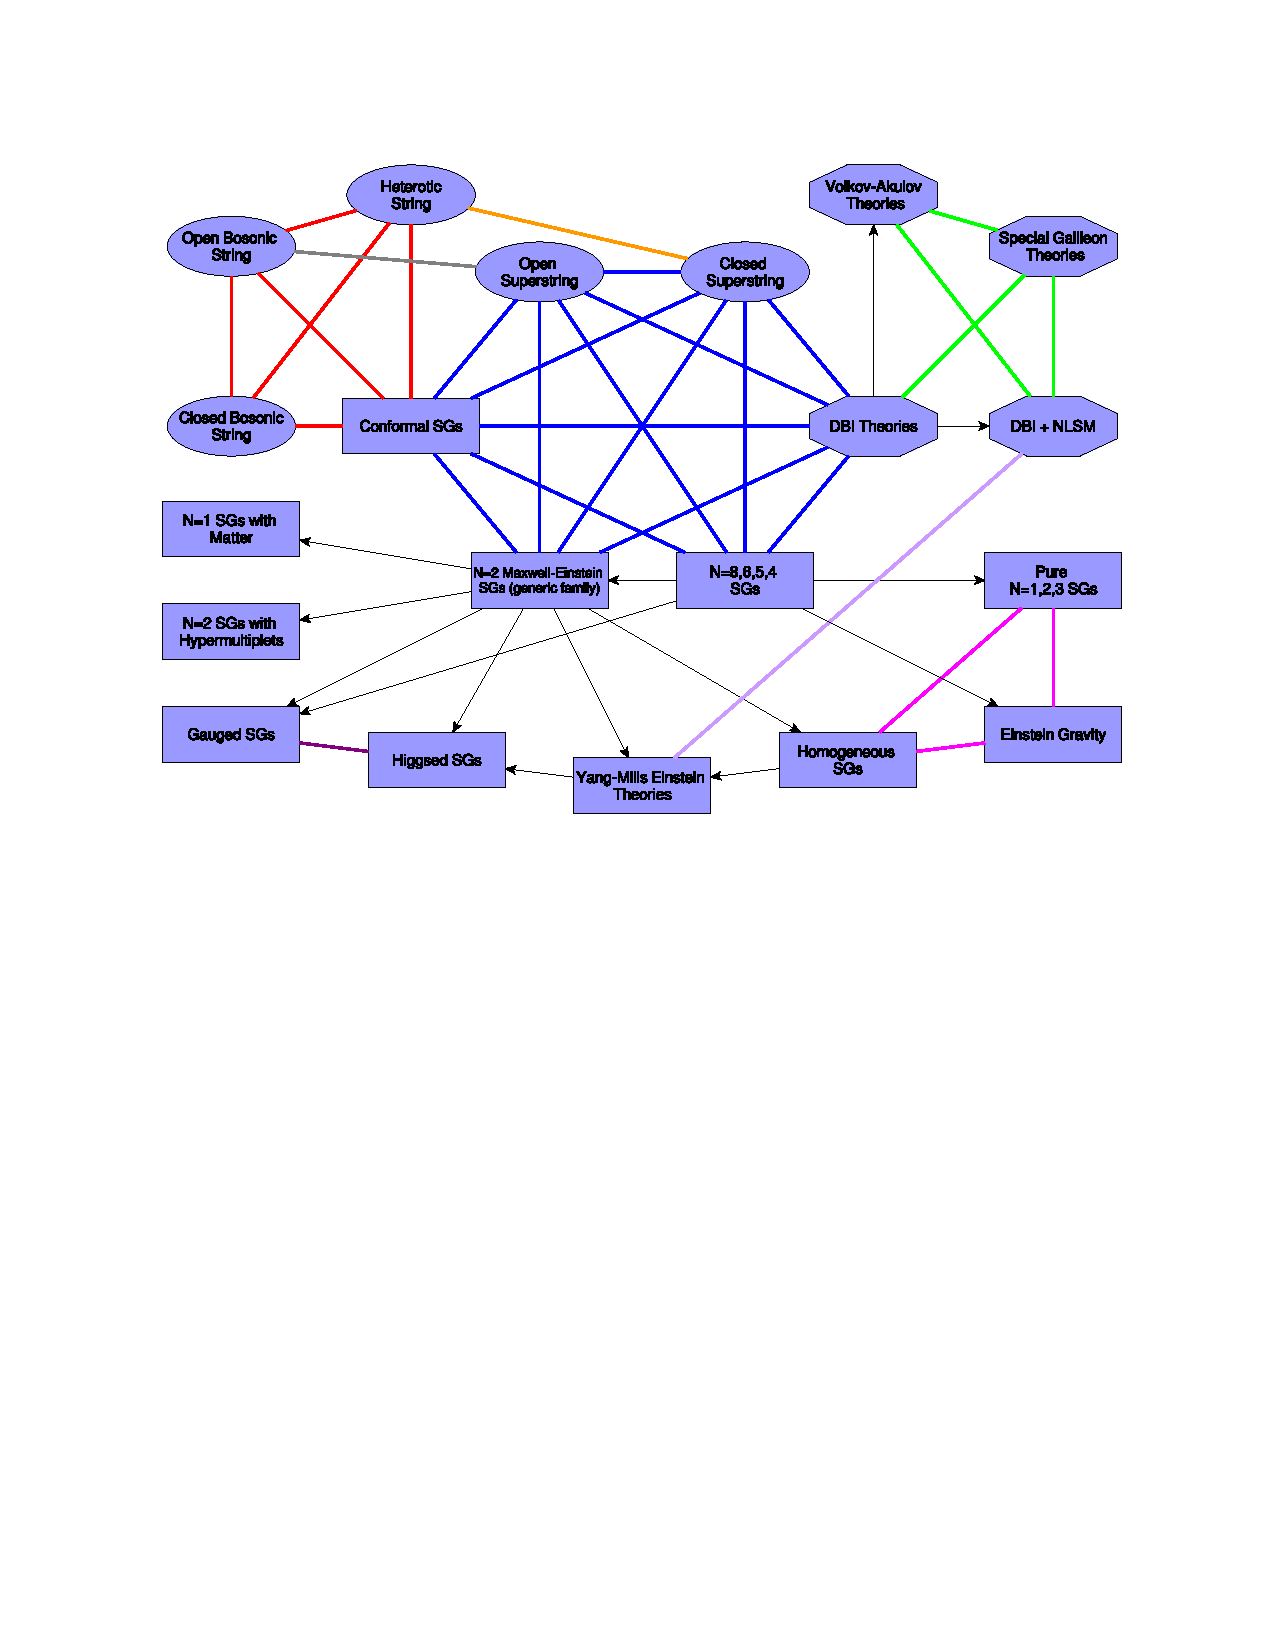
\includegraphics[width=0.85\linewidth]{pic/web.pdf}
	\end{figure}
\end{frame}
\begin{frame}[allowframebreaks]{Del-Dixon-Maltoni basis}
    Using Jacobi identity, $A^\text{YM}$ can be expanded in "half-ladder" basis: \cite{DelDuca:1999rs}
	\begin{small}
		\begin{equation*}
		A^{\text{gauge}}_n=\sum_{\sigma\in S_{n-2}}\overbrace{f^{a_1a_{\sigma_1}b_1}f^{b_1a_{\sigma_2}b_2}\cdots f^{b_{n-3}a_{\sigma_{n-2}}a_n}}^{c_{1\left|\sigma_1\cdots\sigma_{n-2}\right|n}}A_n(1,\sigma_1,\sigma_2,\ldots,\sigma_{n-2},n)
		\end{equation*}
	\end{small}
	\vspace{-8pt}
	\begin{figure}
		\centering
		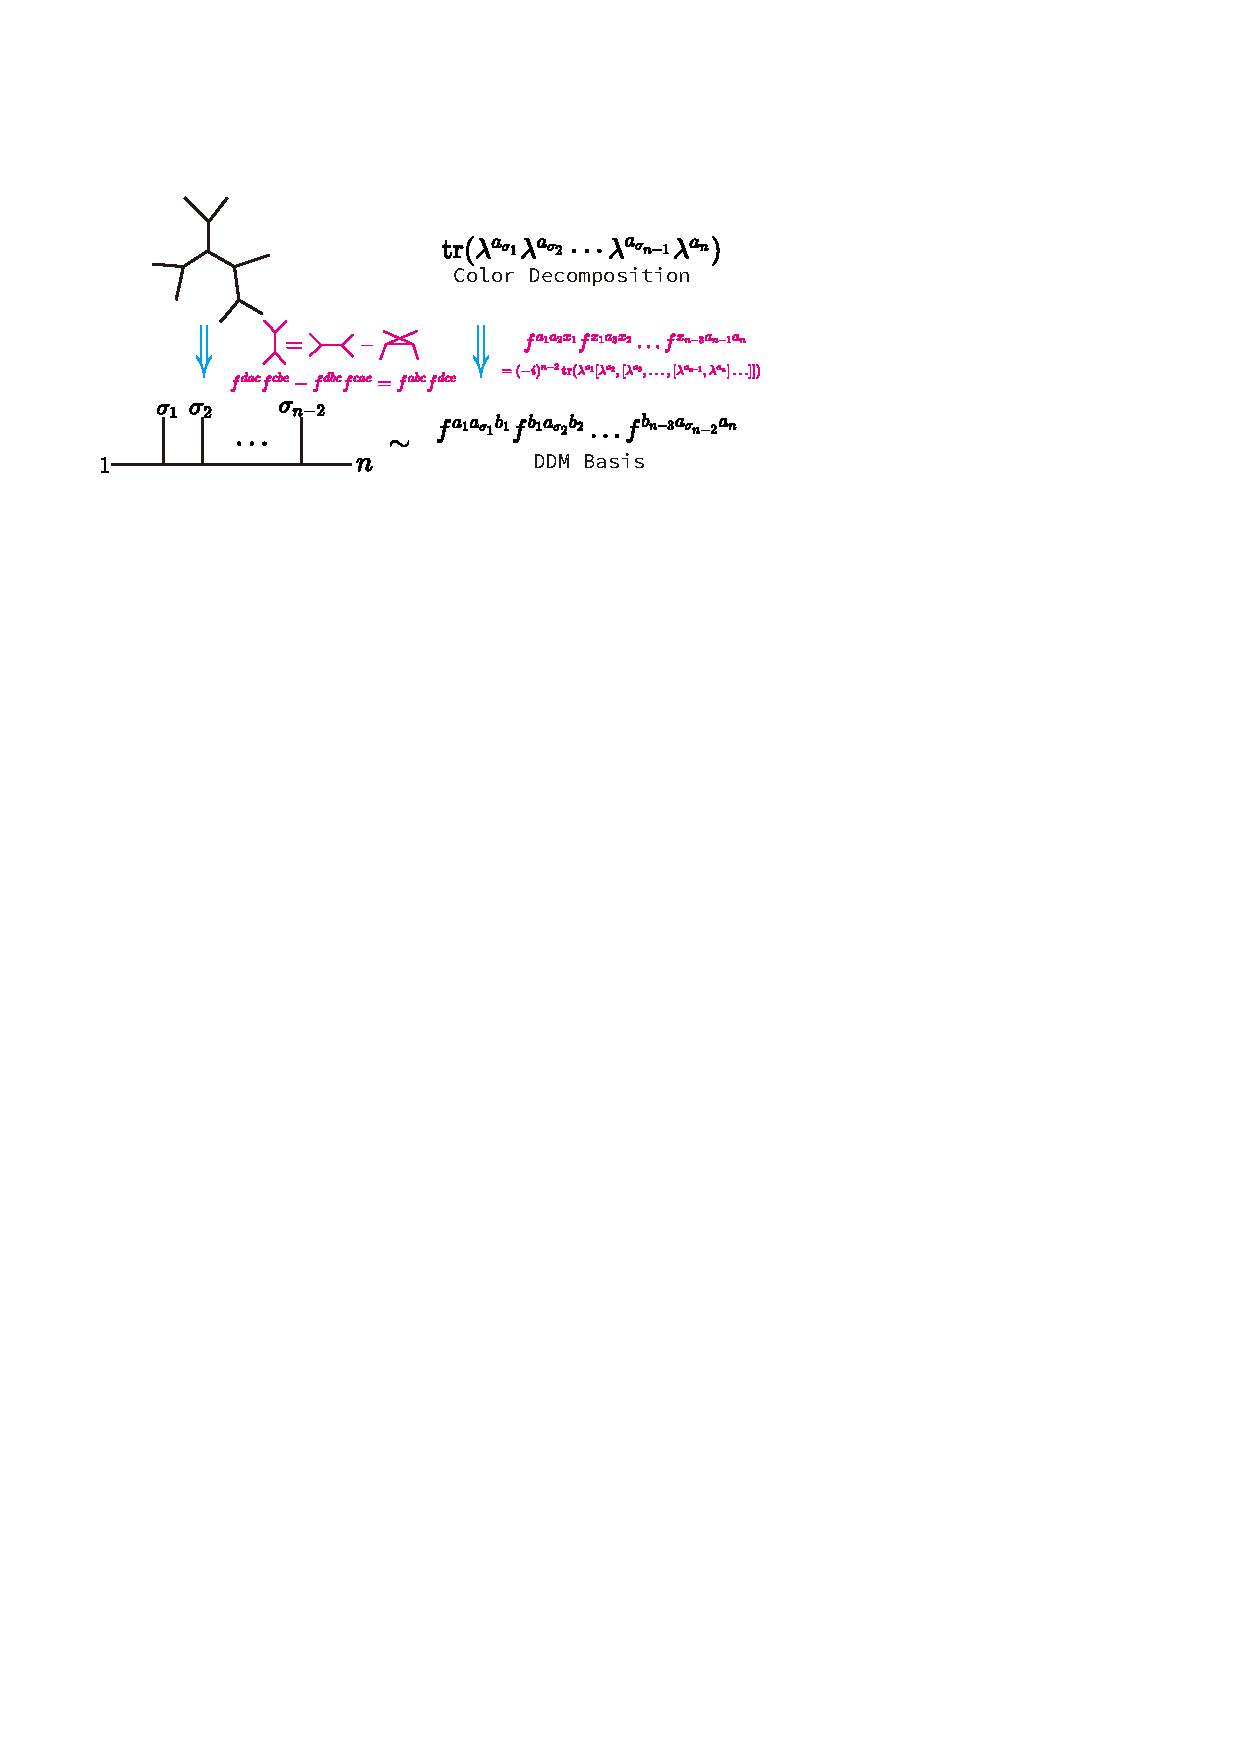
\includegraphics[width=0.85\linewidth]{pic/DDM.pdf}
	\end{figure}
	As discussed in \hyperlink{phi3}{\color{blue}appendix}, $A_n^{\text{gauge}}$ can be rewritten by using partial amplitudes of {\color{WHU} $\tr\phi^3$ theory}, $m(P|Q)$, in DDM basis.
	\begin{equation}\label{eq:ddm}
		\begin{aligned}
			&A^{\text{gauge}}_n=\sum_{ P,Q\in S_{n-2}}c_{1|P|n}m(1,P,n|1,Q,n)N_{1|Q|n}\\
			\Rightarrow& A_n^{\text{gauge}}(P) = \sum_{Q\in S_{n-2}}N_{1|Q|n-1}m(P|1,Q,n-1)
		\end{aligned}
	\end{equation}
	Since in the DDM basis, ${N_{1|Q|n}}$ are independently of each other, they cannot be related through Jacobi identities. If $A^{\text{gauge}}_n$ can be organized in the form above, then the BCJ numerators are naturally constructed. We will see that this is straightforward in the pure spinor formalism.
\end{frame}
\begin{frame}[allowframebreaks]{Construct BCJ numerators}
	To factor out all the $\alpha'$ dependence, the $n$-point open string amplitude \hyperlink{eq:n-pt}{\color{blue}(4)} can be reorganized in terms of $Z$-integral:
	\begin{equation*}
		\mathcal{A}_n(P)=\sum_{AB=23\cdots n-2}\langle V_{1A}V_{(n-1)\tilde{B}}V_n\rangle(-1)^{|B|-1}Z(P|1,A,n,B,n-1)+\mathrm{perm}
	\end{equation*} 
	\begin{equation*}
		Z(P|Q):=(2\alpha^{\prime})^{n-3}\int_{D(P)}\frac{dz_1dz_2\cdots dz_n}{\mathrm{vol}(\mathrm{SL}_2(\mathbb{R}))}\prod_{i<j}^n\left|z_{ij}\right|^{-2\alpha^{\prime}s_{ij}}\mathrm{PT}(Q)
	\end{equation*}
	\begin{equation*}
		P(1,2,\cdots, n):=\frac{1}{z_{12}z_{23}\ldots z_{n-1,n}z_{n,1}}=\frac{1}{z_{n,1}}\mathcal{Z}_{123\cdots n}
	\end{equation*}
	Only one final step remains: taking the $\alpha' \to 0$ limit, one can show that,
	\begin{equation*}
		\lim_{\alpha^{\prime}\to0}Z(P|Q)=m(P|Q),\quad A_n(P)^\mathrm{string}\to A_n(P)^\mathrm{gauge}
	\end{equation*}
	Thus, the open string amplitude reduces to:
	\begin{small}
	\begin{equation*}
		\mathcal{A}_{n}(P)^{\mathrm{string}}\xrightarrow{\alpha^{\prime}\to0}\sum_{AB=23\cdots n-2}{\color{WHU}\langle V_{1A}V_{(n-1)\tilde{B}}V_{n}\rangle(-1)^{|B|-1}}m(P|1,A,n,B,n-1)+\mathrm{perm}
	\end{equation*}
	\end{small}
	Recalling the expression in the DDM basis \hyperlink{eq:ddm}{\color{blue}(5)}:
	\begin{equation*}
		A_n^{\text{gauge}}(P) = \sum_{Q\in S_{n-2}}{\color{WHU}N_{1|Q|n-1}}m(P|1,Q,n-1),\quad \sum_Q\iff\sum_{AnB}+\mathrm{perm}
	\end{equation*}
	we finally obtain:
	\begin{equation*}
		\boxed{N_{1|AnB|n-1}=(-1)^{|B|-1}\langle V_{1A}V_{(n-1)\tilde{B}}V_{n}\rangle}
	\end{equation*}
	More details can be found in \cite{Mafra:2011kj}.
\end{frame}

\section[Comments]{Comments}
\begin{frame}{Conclusion}
	\begin{itemize}
		\item {\color{WHU} The PS superstring allows covariant quantization with manifest target-space SUSY}
		\begin{equation*}
			S_{\mathrm{PS}}=\frac{1}{\pi}\int d^2z\left(\frac{1}{2}\partial X^m\overline{\partial}X_m+p_\alpha\overline{\partial}\theta^\alpha-w_\alpha\overline{\partial}\lambda^\alpha\right)+\mathrm{c.c.}
		\end{equation*}
		\item {\color{WHU} Tree-level amplitudes admit a compact representation in PS superspace}
		{\footnotesize
			\begin{equation*}
				\begin{gathered}
					\mathcal{A}_n(P)=(2\alpha^{\prime})^{n-3}\int d\mu_P^n\sum_{AB=23\ldots n-2}\langle(V_{1A}\mathcal{Z}_{1A})(V_{(n-1)\tilde{B}}\mathcal{Z}_{n-1,\tilde{B}})V_n\rangle+\mathrm{perm}\\
					A_n^{\text{YM}}(P,n)=\sum_{XY=P}\left\langle M_XM_YM_n\right\rangle
				\end{gathered}
			\end{equation*}
		}
		\item {\color{WHU} BCJ numerators can be constructed straightforwardly in the PS formalism*}
		\begin{equation*}
			N_{1|AnB|n-1}=(-1)^{|B|-1}\langle V_{1A}V_{(n-1)\tilde{B}}V_{n}\rangle
		\end{equation*}
	\end{itemize}
\end{frame}
\begin{frame}{Some elementary comments on non-trivial target spacetime}
	% 要有个宇宙安全声明，告诉大家我不是真正的expert，所以这些comment听个乐就好
	% 开场白说：Oh,好的我们现在有纯旋量超弦，或许可以处理R-R flux耦合，乃至解决AdS/CFT猜想引发弦论第三次革命
	% 把阿提亚斯说的话放进去，但是不用放进ppt
	% 讲一下B-RNS-GSS形式也促进了RNS超弦和PS等价性的证明。

	PS Supertstring in $\text{AdS}_{5}\times\text{S}^5$ background can be described by:
	\begin{small}
		\begin{equation*}
		\begin{aligned}
			S_{\text{PS}}=\int d^{2}z&\Bigg[\frac{1}{2}J^{\underline{a}}\bar{J}^{\underline{b}}\eta_{\underline{ab}}+\frac{1}{2}(J^{\alpha}\bar{J}^{\bar{\beta}}-3J^{\bar{\beta}}\bar{J}^{\alpha})\eta_{\alpha\bar{\beta}}\\
			&+\omega_{\alpha}\bar{\nabla}\lambda^{\alpha}+\bar{\omega}_{\bar{\alpha}}\nabla\bar{\lambda}^{\bar{\alpha}}-\frac{1}{2}(N^{ab}\bar{N}_{ab}-N^{a^{\prime}b^{\prime}}\bar{N}_{a^{\prime}b^{\prime}})\Bigg]
		\end{aligned}
	\end{equation*}
	\end{small}
	Covariant vertex operators can also be constructed: \cite{Chandia:2017afc}
	\begin{footnotesize}
		\begin{equation*}
		\begin{aligned}
			V=&\lambda^\alpha\bar{\lambda}^{\bar{\alpha}}A_{\alpha\bar{\alpha}}(g)\\
			U=&2\eta_{\beta\bar{\gamma}}J^{\alpha}\bar{J}^{\beta}{W_{\alpha}}^{\bar{\gamma}}-2\eta_{\gamma\bar{\alpha}}J^{\bar{\alpha}}\bar{J}^{\bar{\beta}}{W^{\gamma}}_{\bar{\beta}}+J^{\alpha}\bar{J}^{\bar{\beta}}A_{\alpha\bar{\beta}}+J^{\alpha}\bar{J}^{\bar{\alpha}}A_{\alpha\underline{a}}-J^{\underline{a}}\bar{J}^{\bar{\alpha}}A_{\underline{a}\bar{\alpha}}\\
			&+\frac{1}{2}J^{\alpha}\bar{N}^{\underline{ab}}F_{\alpha\underline{ab}}-\frac{1}{2}N^{\underline{ab}}\bar{J}^{\bar{\alpha}}F_{ab\bar{\alpha}}+J^{\bar{\beta}}\bar{J}^{\alpha}\bar{\mathcal{V}}_{\alpha\bar{\beta}}+J^{\underline{a}}\bar{J}^{\alpha}\bar{\mathcal{V}}_{\underline{a\alpha}}+J^{\bar{a}}\bar{J}^{\underline{a}}\bar{\mathcal{V}}_{\underline{aa}}+J^{\underline{a}}\bar{J}^{\underline{b}}\mathcal{V}_{\underline{ab}}\\
			&+\frac{1}{4}N^{\underline{ab}}\bar{N}^{\underline{cd}}\mathcal{V}_{\underline{ab}\,\underline{cd}}+\frac{1}{2}N^{\underline{ab}}\bar{J}^{\alpha}\bar{\mathcal{V}}_{\underline{ab}\alpha}+\frac{1}{2}J^{\bar{\alpha}}\bar{N}^{\underline{ab}}\mathcal{V}_{\underline{ab}\bar{\alpha}}+\frac{1}{2}J^{\underline{a}}\bar{N}^{\underline{bc}}\mathcal{V}_{\underline{a}\,\underline{bc}}+\frac{1}{2}N^{\underline{bc}}\bar{J}^{\underline{a}}\bar{\mathcal{V}}_{\underline{a}\,\underline{bc}}
		\end{aligned}
	\end{equation*}
	\end{footnotesize}
	These superfields are constrained by very complicated equations, and further calculation is needed to determine the exact form of $U$ and $V$.
\end{frame}
\begin{frame}{The best of three worlds: B-RNS-GSS formalism}
	PS superstring does not possess world-sheet supersymmetry. Recently the B-RNS-GSS formalism, which combines the desirable features of three formalisms, has attracted considerable attention \cite{Berkovits:2021xwh}.
	\begin{footnotesize}
		\begin{equation*}
			S_{\text{B-RNS-GSS}}=\int d^2z\left(\frac{1}{2}\partial X_m\overline{\partial}X^m+\frac{1}{2}\psi_m\overline{\partial}\psi^m+b\overline{\partial}c+\beta\overline{\partial}\gamma+p_\alpha\overline{\partial}\theta^\alpha+w_\alpha\overline{\partial}\Lambda^\alpha\right)
		\end{equation*}
	\end{footnotesize}
	With the following action in $\text{AdS}_5\times\text{S}^5$ spacetime: \cite{Chandia:2023eel}
	\begin{footnotesize}
		\begin{equation*}
			\begin{aligned}
			&S=\int d^{2}z \Bigg(\frac{1}{2}J_{\underline{a}}\overline{J}^{\underline{a}}+\frac{1}{2}\eta_{\alpha\overline{\alpha}}(J^{\alpha}\overline{J}^{\overline{\alpha}}+J^{\overline{\alpha}}\overline{J}^{\alpha})+d_{\alpha}\overline{J}^{\alpha}+\overline{d}_{\overline{\alpha}}J^{\overline{\alpha}}-\frac{1}{2}\eta^{\alpha\overline{\alpha}}d_{\alpha}\overline{d}_{\overline{\alpha}}+w_{\alpha}\overline{\nabla}\Lambda^{\alpha}\\
			&+\overline{w}_{\overline{\alpha}}\nabla\overline{\Lambda}^{\overline{\alpha}}+ \frac{1}{2}\psi_{\underline{a}}\overline{\nabla}\psi^{\underline{a}}+\frac{1}{2}\overline{\psi}_{\underline{a}}\nabla\overline{\psi}^{\underline{a}}-\frac{1}{2}\psi^{\underline{a}}w_{\alpha}\overline{J}^{\overline{\alpha}}{(\eta\gamma_{\underline{a}})^{\alpha}}_{\overline\alpha}+\frac{1}{2}\overline{\psi}^{\underline{a}}\overline{w}_{\overline{\alpha}}J^{\alpha}{(\gamma_{\underline{a}}\eta)_{\alpha}}^{\overline{\alpha}}-\frac{1}{8}\overline{J}^{\underline{a}}(w\gamma_{\underline{a}}w)\\&\begin{aligned}&- \frac{1}{8}J^{\underline{a}}(\overline{w}\gamma_{\underline{a}}\overline{w})+\frac{1}{2}N^{\left[\underline{ab}\right]}\overline{N}_{\left[\underline{ab}\right]}-\frac{1}{8}\psi^{\underline{a}}\overline{\psi}^{\underline{b}}w_{\alpha}\overline{w}_{\overline{\alpha}}(\gamma_{\underline{a}}\gamma_{\underline{b}}\eta)^{\alpha\overline{\alpha}}-\frac{1}{64}(w\gamma_{\underline{a}}w)(\overline{w}\gamma^{\underline{a}}\overline{w})\Bigg)+S_{\text{gh}}\end{aligned}\end{aligned}
		\end{equation*}
	\end{footnotesize}
	Unintegrated and integrated vertex operators for massless states were constructed in \cite{Chandia:2025nxx}, but they are too complicated to include here.
\end{frame}

\begin{frame}
	\begin{center}
		{\Huge Thanks!}
	\end{center}
	\vspace{0.3cm}
	\begin{figure}[htpb]
	\begin{center}
		
\includegraphics[width=0.6\linewidth]{pic/berkovits.jpg}
		\\
		\vspace{0.1cm}
		\textbf{\color{WHU}With Nathan Berkovits and my friend Chen Huang in String-Math 2025.}
	\end{center}
\end{figure}
	\vspace{0.1cm}
	\begin{center}
	{\huge ありがとうございます}
	\end{center}
\end{frame}

\section[Appendix]{Appendix}
\begin{frame}[allowframebreaks]{Vertext operators in RNS formalism}\label{vertex ops}
	The missing two vertex operators are:
	\begin{equation*}
		\begin{aligned}
			U^{(+\frac{1}{2})}=&\frac{1}{\sqrt{\alpha^{\prime}}}u^{\alpha}\left\{e^{\frac{1}{2}\phi}(i\partial X^{\mu}+\frac{\alpha^{\prime}}{8}(k\cdot\psi)\psi^{\mu})(\Gamma_{\mu})_{\alpha}^{\dot{\beta}}S_{\dot{\beta}}\right\}e^{ik\cdot X}\\
			U^{(0)}=&\sqrt{\frac{2}{\alpha^{\prime}}}\epsilon_{\mu}\left(i\partial X^{\mu}+\frac{\alpha^{\prime}}{2}(k\cdot\psi)\psi^{\mu}\right)e^{ik\cdot X}
		\end{aligned}
	\end{equation*}
	By the way, $S^\alpha$ is called {\color{WHU} spin operator}, which represents one of the most challenging aspects to handle in the RNS formalism.
	
	Indeed, vertex operators connected by a Picture-Changing Operator (PCO) are physically equivalent, as shown here $U^{(-1)}\cong U^{(0)}$ and $U^{(-\frac12)}\cong U^{(+\frac12)}$. However, when computing tree-level correlation functions of vertex operators, the total picture number must sum to $-2$ in order to cancel the contribution from the background superghost number \cite{blumenhagen}.
	
	By the way, you may not be fully familiar with unintegrated and integrated vertex operators. Let me briefly review them. To calculate the string S-matrix, we need to compute correlation functions of the following form:
	\begin{equation*}
		S\sim \frac{1}{V_{\text{CKG}}}\int dz_1\cdots dz_n \left\langle U_1(z_1)\cdots U_n(z_n)\right\rangle
	\end{equation*}
	We call $U_i(z_i)$ the \textcolor{WHU}{integrated vertex operator}, since we must integrate over $z_i$. However, to gauge-fix the conformal Killing group ($V_{\text{CKG}}$) in tree-level, we must also fix three points on the sphere. In this case, $\int \mathrm{d}z U(z)$ at marked points should be replaced by $V(z)$, the \textcolor{WHU}{unintegrated vertex operator}. In the RNS formalism, there is a simple relation between $U$ and $V$, as seen in \hyperlink{eq:UV}{\color{blue}equation (1)}.
\end{frame}
\begin{frame}[allowframebreaks]{Why can we not quantize GS superstring covariantly?}\label{GS}
	To make life easier, let's consider the massless particle limitation of GS superparicle, known as Brink-Schwarz superparticle:
	\begin{equation*}
		S_{\mathrm{BS}}=\int d\tau\left(\Pi^{\mu}P_{\mu}+eP^{\mu}P_{\mu}\right),\quad\Pi^{\mu}:=\dot{X}^{\mu}-\frac{1}{2}\dot{\theta}^{\alpha}\gamma_{\alpha\beta}^{\mu}\theta^{\beta}
	\end{equation*}
	This theory has $\mathcal{N}=1$ supersymmetry:
	\begin{equation*}
		\begin{aligned}
			\delta\theta^{\alpha}&=\epsilon^{\alpha},\quad\delta X^{\mu}=\frac{1}{2}\theta^{\alpha}\gamma_{\alpha\beta}^{\mu}\epsilon^{\beta},\quad\delta P^{\mu}=\delta e=0\\Q_{\alpha}&:=p_{\alpha}-\frac{1}{2}\gamma_{\alpha\beta}^{\mu}\theta^{\beta}P_{\mu},\quad p_{\alpha}:=\frac{\partial L}{\partial\dot{\theta}^{\alpha}}=-\frac{1}{2}\gamma_{\alpha\beta}^{\mu}\theta^{\beta}P_{\mu}
		\end{aligned}
	\end{equation*}
	String theory is a constrained system, much like gauge theory, the worldsheet energy–momentum tensor must vanish. Similarly, in particle theory, we need on-shell condition, $P^2=0$. Moreover, we introduce two pairs of conjugate variables: ${X, P}$ and ${p, \theta}$. The latter are not independent. The constraint between $p$ and $\theta$ is:
	\begin{equation*}
		d_{\alpha}:=p_{\alpha}+\frac{1}{2}\gamma_{\alpha\beta}^{\mu}\theta^{\beta}P_{\mu}=0
	\end{equation*}
	It is straightforward to compute their Poisson brackets:
	\begin{equation*}
		\{d_\alpha,d_\beta\}_{\mathrm{PB}}=-\gamma_{\alpha\beta}^\mu P_\mu
	\end{equation*}
	A more careful analysis shows that these constraints consist of 8 first-class and 8 second-class constraints. Only in light-cone coordinates do these two classes decouple:
	\begin{equation*}
		\{d_\alpha,d_\beta\}_{\mathrm{PB}}=-\gamma_{\alpha\beta}^-P^+\propto\begin{pmatrix}1_{8\times8}&0_{8\times8}\\\\0_{8\times8}&0_{8\times8}\end{pmatrix}
	\end{equation*}
	Dirac’s classification of constraints is a very old concept \cite{dirac}:
	\begin{itemize}
		\item {\color{WHU} First class: $\{d_1, d_2\}=0$}\\
		Corresponds to gauge symmetries. Can be eliminated by gauge fixing or via Gupta–Bleuler quantization: $d\ket{\text{phys}} = 0$.
		\item {\color{WHU} Seconed class: $\{d_1,d_2\}\neq 0$}\\
		Corresponds to redundant degrees of freedom\footnote{Such as using $(x, y, z)$ to describe a planar motion.}. Before canonical quantization, Poisson brackets must be replaced by {\color{WHU}Dirac brackets}. The constraint $d = 0$ is then treated as a strong operator equation: $\hat{d} = 0$.\footnote{Don't need to act on $\ket{\text{phy}}$}
	\end{itemize}
	Furthermore, GS formalism has an additional gauge symmetry, {\color{WHU}$\kappa$-symmetry}:
	\begin{equation*}
		\delta\theta^{\alpha}=P^{\mu}\gamma_{\mu}^{\alpha\beta}\kappa_{\beta},\quad\delta X^{\mu}=-\frac{1}{2}\theta^{\alpha}\gamma_{\alpha\beta}^{\mu}\delta\theta^{\beta},\quad\delta P^{\mu}=0,\quad\delta e=\dot{\theta}^{\alpha}\kappa_{\alpha}
	\end{equation*}
	This symmetry can be fixed in light-cone coordinates, after which the full theory can be quantized. For further details, see \cite{Berkovits:2017ldz}.
\end{frame}
\begin{frame}{Linearized 10D SYM superfields: equation of motion}\label{10d sym}
	In 10D SYM, the physical spectrum contains only gluons 
	$\mathbb{A}_\mu=\mathbb{A}_\mu(X,\theta)$ and gluinos 
	$\mathbb{A}_\alpha=\mathbb{A}_\alpha(X,\theta)$, satisfying the following e.o.m:
	\begin{equation*}
		\begin{aligned}
			\{\nabla_{\alpha},\nabla_{\beta}\}&=\gamma_{\alpha\beta}^{\mu}\nabla_{\mu},&\{\nabla_{\alpha},\nabla_{\mu}\}&=-(\gamma_{\mu}\mathbb{W})_{\alpha},\\
			\{\nabla_{\alpha},\mathbb{W}^{\beta}\}&=\frac{1}{4}(\gamma^{\mu\nu})_\alpha{}^\beta\mathbb{F}_{\mu\nu},&[\nabla_\alpha,\mathbb{F}^{\mu\nu}]&=(\mathbb{W}^{[\mu}\gamma^{\nu]})_\alpha
		\end{aligned}
	\end{equation*}
	\begin{equation*}
		\begin{gathered}
			\mathbb{F}_{\mu\nu}:=-\left[\nabla_\mu,\nabla_\nu\right],\quad\mathbb{W}_\mu^\alpha:=\left[\nabla_\mu,\mathbb{W}^\alpha\right]\\
			\nabla_{\alpha}=D_{\alpha}-\mathbb{A}_{\alpha},\quad\nabla_{\mu}=\partial_{\mu}-\mathbb{A}_{\mu},\quad D_{\alpha}=\frac{\partial}{\partial\theta^{\alpha}}+\frac{1}{2}(\gamma^{\mu}\theta)_{\alpha}\partial_{\mu}
		\end{gathered}
	\end{equation*}
	In the linearized approximation, superfields $\mathbb{K}\mapsto K$ describe asymptotic states and satisfy:
	\begin{equation*}
		\begin{aligned}
			D_{\alpha}A_{\beta}^{i}+D_{\beta}A_{\alpha}^{i}&=\gamma_{\alpha\beta}^{\mu}A_{\mu}^{i},\quad D_{\alpha}A_{\mu}^{i}=(\gamma_{\mu}W_{i})_{\alpha}+\partial_{\mu}A_{\alpha}^{i},\\D_{\alpha}W_{i}^{\beta}&=\frac{1}{4}(\gamma^{\mu\nu})_{\alpha}{}^{\beta}F_{\mu\nu}^{i},\quad D_{\alpha}F_{\mu\nu}^{i}=\partial_{[\mu}(\gamma_{\nu]}W_{i})_{\alpha}
		\end{aligned}
	\end{equation*}
\end{frame}
\begin{frame}[allowframebreaks]{Linearized 10D SYM superfields: $\theta$-expansion}
	In the Harnad–Shnider gauge, $\theta^\alpha A_\alpha=0$, these equations can be solved explicitly. 
	The resulting superfields admit a $\theta$-expansion. For pure spinor computations it suffices to keep 
	terms up to $\mathcal{O}(\theta^4)$:
	\begin{footnotesize}
		\begin{equation*}
		\begin{aligned}
			A^i_\alpha(X,\theta) &= 
			\Biggl\{
			\frac{1}{2} (\theta \gamma_m)_\alpha e_i^m
			+ \frac{1}{3} (\theta \gamma_m)_\alpha (\theta \gamma^m \chi_i)
			- \frac{1}{32} (\theta \gamma^m)^\alpha (\theta \gamma_{mnp}\theta) f_i^{np} \\
			&+ \frac{1}{60} (\theta \gamma^m)_\alpha (\theta \gamma_{mnp}\theta) k_i^n (\chi_i \gamma^p \theta)
			+ \frac{1}{1152} (\theta \gamma^m)_\alpha (\theta \gamma_{mnp}\theta) (\theta {\gamma^p}_{qr}\theta) k_i^n f_j^{qr}
			+ \cdots
			\Biggr\} e^{k_i \cdot X},\\
			A^m_i(X,\theta) &= 
			\Biggl\{
			e_i^m
			+ (\theta \gamma^m \chi_i)
			- \frac{1}{8} (\theta {\gamma^m}_{pq}\theta) f_i^{pq}
			+ \frac{1}{12} (\theta {\gamma^m}_{np}\theta) k_i^n (\chi_i \gamma^p \theta) \\
			&+ \frac{1}{192} (\theta {\gamma^m}_{nr}\theta)(\theta {\gamma^r}_{pq}\theta) k_i^n f_i^{pq}
			- \frac{1}{480} (\theta {\gamma^m}_{nr}\theta)(\theta {\gamma^r}_{pq}\theta) k_i^n k_i^p (\chi_i \gamma^q \theta) 
			+ \cdots
			\Biggr\} e^{k_i \cdot X},
		\end{aligned}
	\end{equation*}
	\end{footnotesize}
	\begin{footnotesize}
	\begin{equation*}
		\begin{aligned}
			W^\alpha_i(X,\theta) =& 
			\Biggl\{
			\chi_i^\alpha
			+ \frac{1}{4} (\theta \gamma_{mn})^\alpha f_i^{mn}
			- \frac{1}{4} (\theta \gamma_{mn})^\alpha k_i^m (\chi_i \gamma^n \theta)
			- \frac{1}{48} (\theta \gamma_m{}^q)^\alpha (\theta \gamma_{qnp}\theta) k_i^m f_i^{np} \\
			+ \frac{1}{96} (\theta \gamma_m{}^q)^\alpha& (\theta \gamma_{qnp}\theta) k_i^m k_i^n (\chi_i \gamma^p \theta)
			- \frac{1}{1920} (\theta \gamma_m{}^r)^\alpha (\theta {\gamma_{nr}}^s\theta)(\theta \gamma_{spq}\theta) k_i^m k_i^n f_i^{pq}
			+ \cdots
			\Biggr\} e^{k_i \cdot X},\\
			F^{mn}_i(X,\theta) = &
			\Biggl\{
			f_i^{mn}
			- k_i^{[m} (\chi_i \gamma^{n]} \theta)
			+ \frac{1}{8} (\theta \gamma_{pq}{}^{[m}\theta) k_i^{n]} f_i^{pq}
			- \frac{1}{12} (\theta \gamma_{pq}{}^{[m}\theta) k_i^{n]} k_i^p (\chi_i \gamma^q \theta) \\
			-\frac{1}{192}&(\theta{\gamma_{ps}}^{[m}\theta)k_i^{n]}k_i^pf_i^{qr}(\theta{\gamma^s}_{qr}\theta)+\frac{1}{480}(\theta{\gamma^{[m}}_{ps}\theta)k_i^{n]}k_i^pk_i^q(\chi_i\gamma^r\theta)(\theta{\gamma^s}_{qr}\theta)
			+ \cdots
			\Biggr\} e^{k_i \cdot X}.
		\end{aligned}
	\end{equation*}
	\end{footnotesize}
	Here we use the convention $ik \mapsto k$ to get rid of $i=\sqrt{-1}$. Moreover,
	\begin{equation*}
		f_i^{\mu\nu}:=k_i^\mu e_i^\nu-k_i^\nu e_i^\mu
	\end{equation*}
	$e^m$ is the polarization vector for boson and $\chi^\alpha$ is the wavefunction of fermion.
\end{frame}
\begin{frame}[allowframebreaks]{3-pt amplitude}\label{3-pt}
	To compute the disk amplitudes \hyperlink{disk}{\color{blue}(3)}, we encounter nested correlators. The inner correlator is handled by OPEs, which reduce the double bracket to $\langle V^3\rangle$. The remaining step is to integrate over zero modes. The 3-point amplitude is chosen here because it receives no OPE contributions and is determined entirely by the zero modes of $\lambda_\alpha$ and $\theta^\alpha$.
	\begin{equation*}
		\begin{aligned}\mathcal{A}(1,2,3)&=\left\langle V_1 V_2 V_3\right\rangle=\langle(\lambda A_1)(\lambda A_2)(\lambda A_3)\rangle\\&=\mathcal{A}(1_b,2_b,3_b)+\mathcal{A}(1_b,2_f,3_f)+\mathcal{A}(1_f,2_b,3_f)+\mathcal{A}(1_f,2_f,3_b)
		\end{aligned}
	\end{equation*}
	The second equality shows that in the PS formalism we compute superamplitudes directly, and the components must then be extracted by hand.
	
	To evaluate the outer bracket, we use the following PS superspace measure:
	\begin{equation}
		(\lambda^3\theta^5):=(\lambda\gamma^m\theta)(\lambda\gamma^n\theta)(\lambda\gamma^p\theta)(\theta\gamma_\mathrm{mnр}\theta),\quad \left\langle(\lambda^3\theta^5)\right\rangle = 2880
	\end{equation}
	{\color{WHU} Note: }{The value $2880$ is conventional, it can be absorbed into the definition of the string coupling, so any choice is acceptable.}
	
	Next, we use the $\theta$-expansion of the superfields. For our purpose:
\begin{footnotesize}
		\begin{equation*}
		\lambda^\alpha A_\alpha(X,\theta)\to\left\{\frac{1}{2}e_m(\lambda\gamma^m\theta)-\frac{1}{32}f_{mn}(\lambda\gamma_p\theta)(\theta\gamma^\mathrm{mnр}\theta)-\frac{1}{3}(\lambda\gamma_m\theta)(\theta\gamma^m\chi_i)\right\}e^{k\cdot X}
	\end{equation*}
\end{footnotesize}
	For the 3-gluon component amplitude, only the first two bosonic terms contribute. There are three possibilities: $(\theta^3,\theta^1,\theta^1)$, $(\theta^1,\theta^3,\theta^1)$ and $(\theta^1,\theta^1,\theta^3)$:
	\begin{equation*}
		\mathcal{A}(1_b,2_b,3_b)=-\frac{1}{128}e_1^mf_2^{pq}e_3^n\langle(\lambda\gamma^m\theta)(\lambda\gamma^r\theta)(\lambda\gamma^n\theta)(\theta\gamma_{pqr}\theta)\rangle+\mathrm{cyc}(1,2,3)
	\end{equation*}
	With some magical $\gamma$-matrix identities, one can show:
	\begin{equation*}
		\langle(\lambda\gamma^m\theta)(\lambda\gamma^r\theta)(\lambda\gamma^n\theta)(\theta\gamma_{pqr}\theta)\rangle=24\delta_{pqr}^{mrn}\xlongequal{\tr\delta = 10}-64\delta_{pq}^{mn}
	\end{equation*}
	It has been proved that any $(\lambda^3\theta^5)$ can be reduced to the standard form \hyperlink{l3t5}{\color{blue}(6)}. An efficient \texttt{FORM} package is available for this purpose \cite{Mafra:2010pn}.
	
	Thus, the 3-gluon amplitude becomes:
	\begin{equation*}
		\mathcal{A}(1_b,2_b,3_b)=\frac{1}{2}e_1^mf_2^{mn}e_3^n+\mathrm{cyc}(1,2,3)=(e_1\cdot k_2)(e_2\cdot e_3)+\mathrm{cyc}(1,2,3)
	\end{equation*}
	That's what we all learned back in kindergarten. Similarly, one can check that the amplitude for one gluon and two gluinos is:
	\begin{equation*}
		\mathcal{A}(1_b,2_f,3_f)=\frac{1}{18}e_1^m\langle(\lambda\gamma_m\theta)(\lambda\gamma_n\theta)(\lambda\gamma_p\theta)(\theta\gamma^n\chi_2)(\theta\gamma^p\chi_3)\rangle=e_1^m(\chi_2\gamma_m\chi_3)
	\end{equation*}
	Here the following Fierz identity is useful:
	\begin{equation*}
		\theta^\alpha\theta^\beta=\frac{1}{96}\gamma_{rst}^{\alpha\beta}(\theta\gamma^{rst}\theta)
	\end{equation*}
\end{frame}
\begin{frame}{$\tr\phi^3$ theory}\label{phi3}
	$\tr\phi^3$ theory is described by the Lagrangian:
	\begin{equation*}
		\mathcal{L}_{\phi^{3}}=\frac{1}{2}\partial_{m}\Phi_{i|a}\partial^{m}\Phi_{i|a}+\frac{1}{3!}f_{ijk}\tilde{f}_{abc}\Phi_{i|a}\Phi_{j|b}\Phi_{k|c}
	\end{equation*}
	The $n$-point amplitude takes the form \cite{Cachazo:2013iea}:
	\begin{equation*}
		A_n^{\phi^3}=\sum_{i\in\Gamma_n}\frac{c_i\tilde{c_i}}{D_i}=\sum_{P,Q\in S_{n-2}}c_{1|P|n}m(1,P,n|1,Q,n)\tilde{c}_{1|Q|n}
	\end{equation*}
	The second equality follows purely from Jacobi identities among $\{c_i\}$. Since BCJ numerators $\{N_i\}$ obey the same Jacobi identities as $\{\tilde{c}_i\}$, one expects:
	\begin{equation*}
		A_n^\mathrm{gauge}=\sum_{P,Q\in S_{n-2}}c_{1|P|n}m(1,P,n|1,Q,n)N_{1|Q|n}
	\end{equation*}
	The partial amplitudes $m(P|Q)$ and their string-theoretic analogues can be computed via graphical rules \cite{Mizera:2016jhj}.
\end{frame}

% ==== 参考文献列表 ====
\begin{frame}[allowframebreaks]
\printbibliography
\end{frame}

\end{document}